%===================================== CHAP 4 =================================

\chapter{Experiments and results}\label{chpt:experiments}

This chapter begins with a fairly thorough analysis of the hippocampal module. In this analysis several variables are chosen as free variables, for which traditional experiments testing the variables (schemes and configurations) are run. Novel aspects are proposed and implemented according to the attained results, and even further experiments are proposed, performed and analysed.

Following the analysis of the hippocampal module is memory consolidation to the neocortical network for several of the schemes from the previous section in the hippocampal model, i.e. learning by chaotically recalled patterns and optionally through pseudopatterns.

This chapter structures experiments into sub-sections, which also contain a (detailed and somewhat abstract) analysis of the specific experiment results. The research questions, and a more general and abstract discussion, is addressed in the next chapter, \ref{chpt:discussion}.
Roughly speaking, the free variables which are tested in the experiments are initially asynchronous and synchronous updating of the CA3-layer within the hippocampal model, followed by the dentate gyrus (DG) weighting, two different neuronal turnover modes, and the neuronal turnover rating itself.


\section{Setup}

Initially, the setup was as follows,

\begin{table}
\centering
\caption{Lists the number of neurons in each layer within the hippocampal module.}
\label{table:number_of_neurons}
\begin{tabular}{l|l|l|l|l|l|}
\cline{2-6}
                              & Input & EC  & DG   & CA3 & Output \\ \hline
\multicolumn{1}{|l|}{Neurons} & 49    & 240 & 1600 & 480 & 49     \\ \hline
\end{tabular}
\end{table}

\begin{table}
\centering
\caption{Displaying the firing rates for the different layers, and the resulting values $k$ for k-Winners-Takes-All.}
\label{table:firing_rates}
\begin{tabular}{l|l|l|l|}
\cline{2-4}
                                  & EC   & DG   & CA3  \\ \hline
\multicolumn{1}{|l|}{Firing rate} & 0.10 & 0.01 & 0.04 \\ \hline
\multicolumn{1}{|l|}{Resulting $k$} & 24 & 16 & 19 \\ \hline
\end{tabular}
\end{table}

% initial weight distribution - Gaussians
\begin{table}[]
\centering
\caption{Displaying the parameters for $\mu$ and $\sigma^2$, with which the weights are normally distributed. Note that the parameters found in the table correspond to the tuple $(\mu, \sigma^2)$.}
\label{table:initial_weight_distributions}
\begin{tabular}{l|l|l|l|}
\cline{2-4}
                          & DG        & CA3       & Out      \\ \hline
\multicolumn{1}{|l|}{EC}  & (0.5, 0.25) & (0.5, 0.25) & n/a      \\ \hline
\multicolumn{1}{|l|}{DG}  & n/a       & (0.9, 0.01) & n/a      \\ \hline
\multicolumn{1}{|l|}{CA3} & n/a       & (0.5, 0.25) & (0.0, 0.5) \\ \hline
\end{tabular}
\end{table}

The neuronal turnover rate, together with the weighting of the connections from DG during learning, were parameters that were calibrated during preliminary of experiments. The data which was empirically obtained are summarised in figures below in chapter \ref{section:experiments}, after the experimental details have been outlined. Initially, the parametrization of the model settings were that of the DG-weighting being set to $25.0$, and the neuronal turnover rate to $0.50$, see \ref{table:initial_settings} for further constant parameters.

\begin{table}
\centering
\caption{Initial model variable constant settings. Neuronal turnover was calibrated through initial experiments along with the CA3 neuronal updating scheme, as well as the DG-weighting.}
\label{table:initial_settings}
\begin{tabular}{|l|l|l|l|l|l|l|l|l|l|}
\cline{1-8}
Parameter: & Gamma & Epsilon & Nu   & k\_m & k\_r & a\_i & alpha \\ \hline
Value:     & 0.70  & 100.0   & 0.10 & 0.10 & 0.95 & 0.80 & 2.00 \\ \hline
\end{tabular}
\end{table}


% ========================== EXPERIMENTS ============================          
\section{Experiments}\label{section:experiments}

Before I introduce experiments designed to test specific aspects of the model, along with aggregate results such as graphs of mean convergence ratios, I would like quickly introduce the model functionality at a slightly lower and more detailed level. The intention of this is to create a more complete and sound picture of the model elements, as well as to provide the reader with a more thorough understanding of the representations that are used as input and output data. 

% \subsection{Data set}
As previously mentioned, the input and output layers consist of 49 neurons each. (I MIGHT perform some experiments for 200 I/O with correlated patterns for some config.s later on, in that case: Refactor then). Now, for the actual input and output data, the same I/O patterns as outlined in \citep{Hattori2010, Hattori2014} is used. That is, two sets of 25 distinct patterns are used, namely the first 25 letters of the alphabet in uppercase for the first set, and in lower case for the second. Each letter is compressed to a 7x7 image of binary pixel values (black or white), in other words bipolar vectors of length 49, where -1 corresponds to black, and 1 to white. Note that the input and output space is significantly reduced by constraining the vectors to bipolar values. (more specifics on this?)

\begin{figure}\label{fig:sample_letters}
    \centering
    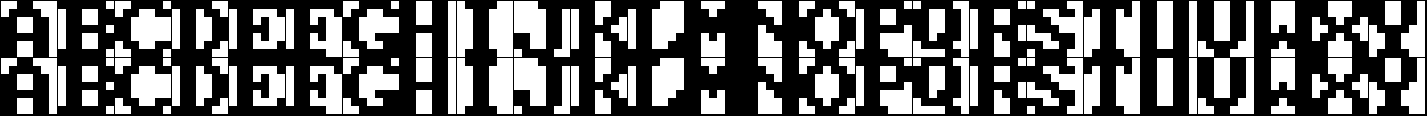
\includegraphics[width=9cm]{fig/im_both.png}
    \caption{Illustrating the 7x7 images that are used as input and output patterns, the first row being the input patterns and the second being the associated output pattern, here illustrated for an autoassociative case, which is used in the initial experimentation.}
\end{figure}

Following is a demonstration of hippocampal model learning, with figures of model output after each learning iteration for chaotic recall and normal recall, i.e. pattern associations. The two first subsets of autoassociative patterns, that is \{A$\rightarrow$A, B$\rightarrow$B\}, and \{C$\rightarrow$C, D$\rightarrow$D\}, are used as training sets in this example.
Furthermore, the hippocampal module is instantiated with the parameter values as outlined above in tables \ref{table:initial_settings} and \ref{table:firing_rates}, a neuronal turnover rate $\tau = 0.04$, and a DG-weighting of $25$. Neuronal turnover is performed between every learnt training set - that is, only once after learning the \{A$\rightarrow$A, B$\rightarrow$B\} associations, before commencing learning of the two next. Here the convergence criteria is set to a static number of training iterations, equal to $15$, while in the experiments, results are generated and analysed for both a dynamic convergence criteria for both learning and stability during recall, as well as for two configurations of $i$ training iterations for convergence and 'stable' recall. Furthermore, the weight matrices are instantiated according to their respective firing rates, with weights being randomly assigned according to Gaussian distributions using the parameters in table \ref{table:initial_weight_distributions}, for a number of neurons corresponding to the layers' firing rates (as outlined in table \ref{table:firing_rates}).

Instantiating the hippocampal model using the parametrization as outlined above, I generated images of the network output for pattern recall (i.e. associations), and chaotic recall for every training iteration. These were generated using both synchronous, and asynchronous updating of the CA3-layer of the model.

\begin{figure}
    \centering
    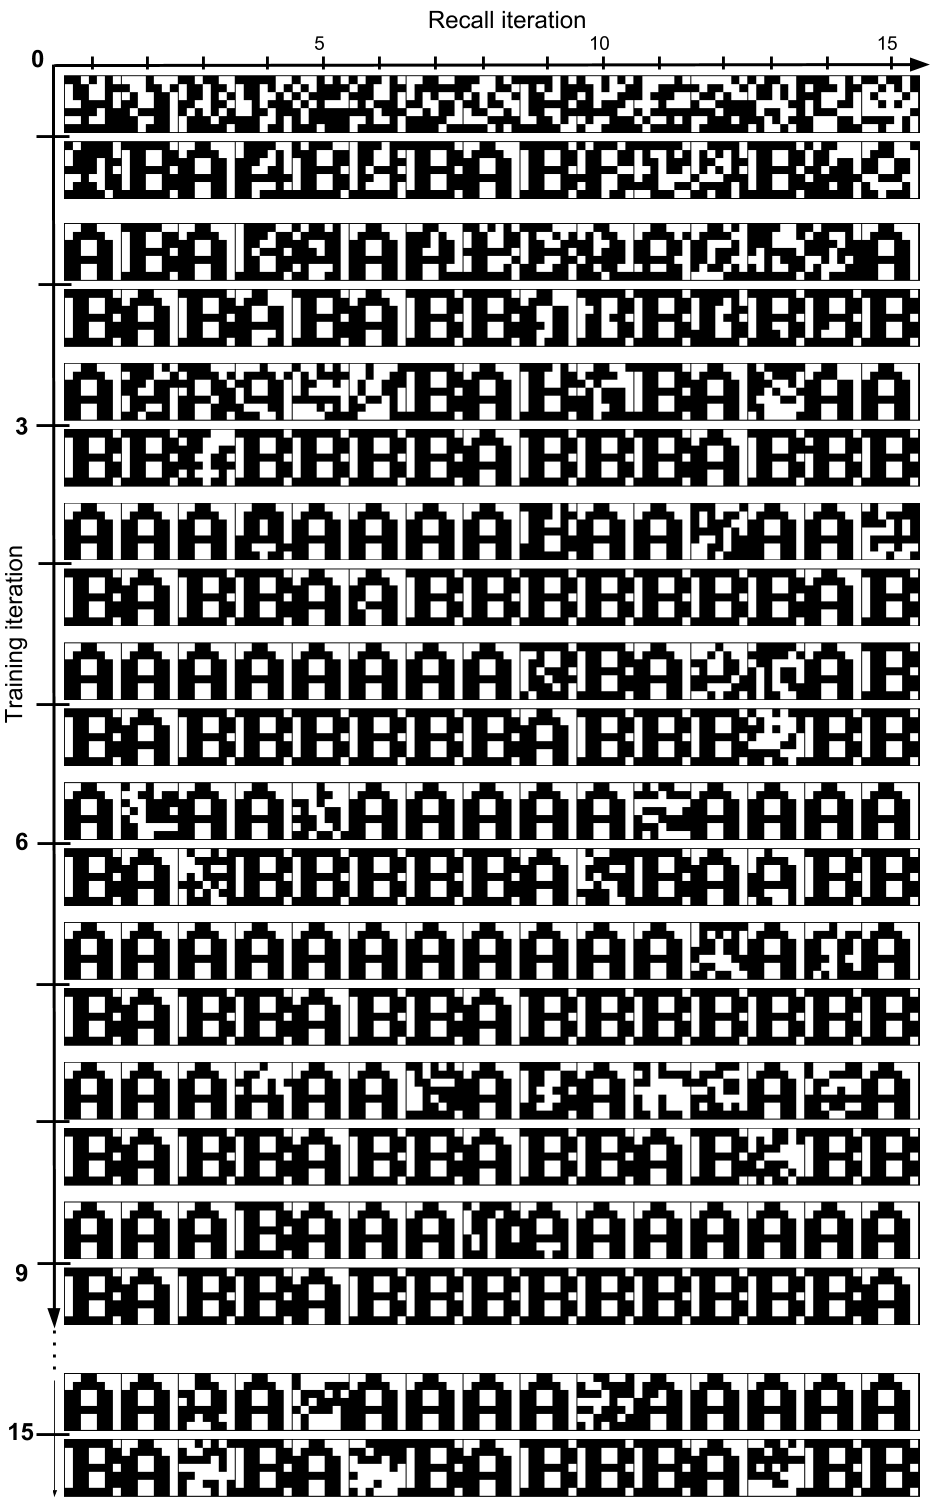
\includegraphics[width=11cm]{fig/AB-pattern-associations-sync-tm0-dgw25}
    \caption{Displaying the recalled pattern for inputs A for the upper row, and B for the lower row, for every learning iteration.}
    \label{fig:pattern_associations_sync}
\end{figure}

\begin{figure}
    \centering
    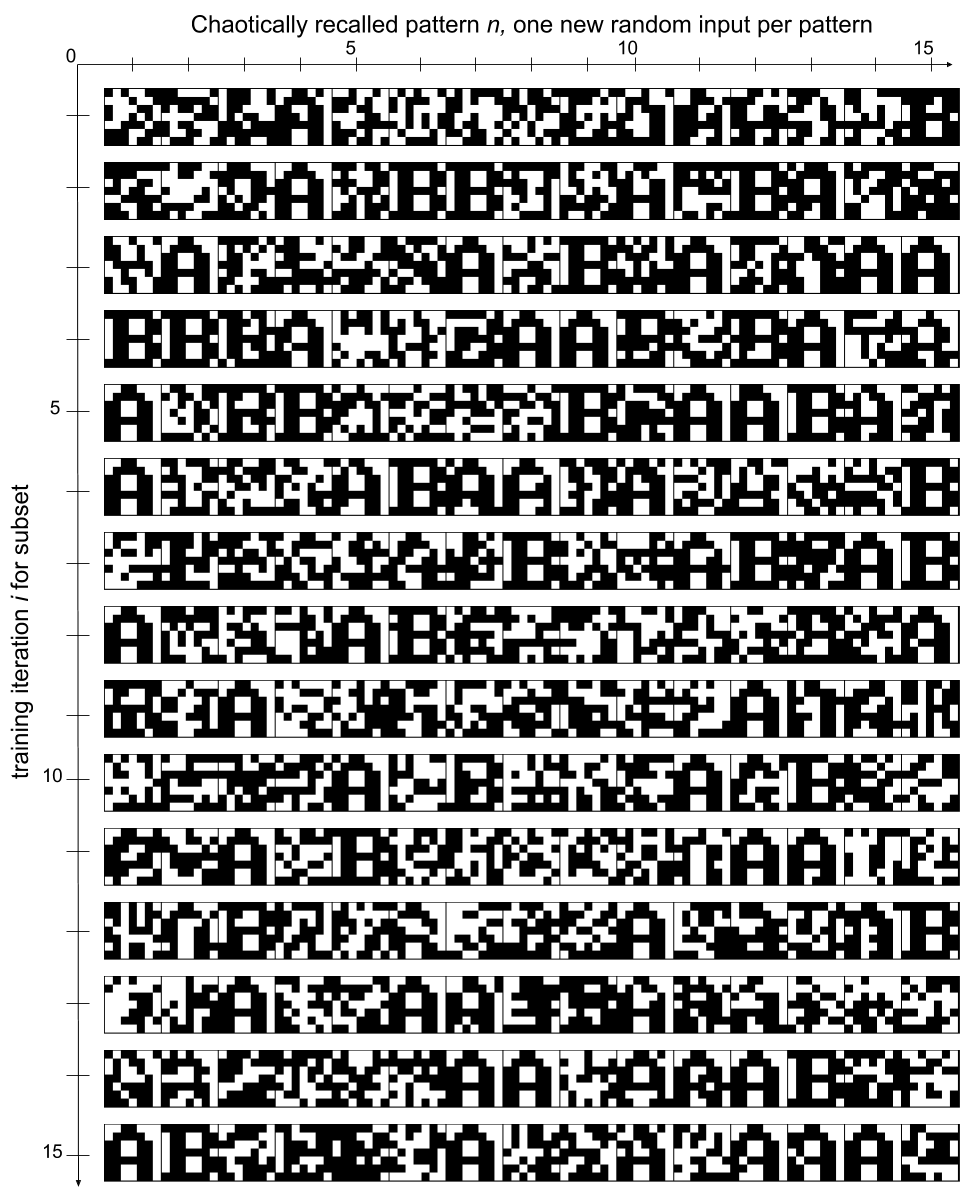
\includegraphics[width=12cm]{fig/AB-chaotic-recall-sync-tm0-dgw25}
    \caption{Displaying the patterns which were recalled by chaotic recall - that is, for each training iteration, 15 patterns were recalled. For each pattern that was recalled, a (new) random input was generated and set as the model's input. Note also that using the same random input also would yield chaotically recalled patterns, which is also included in the trials and experiments contained later in this chapter.}
    \label{fig:chaotic_recall_sync}
\end{figure}

When considering the two figures (\ref{fig:pattern_associations_sync}, \ref{fig:chaotic_recall_sync}) that display the recalled patterns during and after learning pattern-associations for patterns A$\rightarrow$A, and B$\rightarrow$B, it seems that pattern separation is unsuccessful, as the output for input letters A and B remains unstable. Furthermore, this instability is exemplified by the chaotically recalled patterns, which barely recalls the letters A and B, and mostly only spurious patterns that do not resemble the original input nor output patterns. Pattern separation is one of the aspects that are evaluated in this thesis. It is evaluated through successful convergence in the first configurations where the convergence criteria is defined as the output being stable for three iterations of recall. Furthermore, it is analysed in terms of all the configurations by considering the perfect recall rates, as well as spurious pattern recall rates.

In order to demonstrate a more succesful configuration at the low level, an example using (XX) is included below:

\begin{figure}
    \centering
    \includegraphics[width=12cm]{fig/}
    \caption{DEMONSTRATING DON DADA ON THE DOWNLOAD}
\end{figure}

\subsection{Experiment 1: Updating scheme of CA3 and Neuronal Turnover}

In order to evaluate the impact of the way in which action potential is propagated and synaptic connection strength modification occurs, i.e. the order of neuronal activation value updates and weight modification, two updating schemes were used. Namely updating the neuronal activation values synchronously, reducing the propagation of values from one layer of neurons to another to a set of vector and matrix operations, or asynchronously, requiring updating each and every neuron independently. In the simplest case of synchronous updating, i.e. for all non-chaotic layers, the synchronous propagation scheme is simply reduced to a vector of activation values multiplied by a weight matrix, which is adjusted through an activation function.

\subsection{Experiment 2: Hippocampal model calibration}
\subsubsection{Methods}
\subsubsection{Results}

\subsection{Experiment 3: Extracting auto-associative patterns by chaotic recall}
\subsection{Experiment 4: Extracting hetero-associative patterns by chaotic recall}

\subsection{Experiment 5: Consolidation performance, experiment 3}
\subsection{Experiment 6: Consolidation performance, experiment 4}

\subsection{Experiment Y: Novel}


% ========================== RESULTS ============================
\section{Results}

\subsection{Experiment 1: The updating scheme of CA3 and Neuronal Turnover}
% \subsubsection{Synchronous updating}

% \begin{figure}[h!]
%     \centering
%     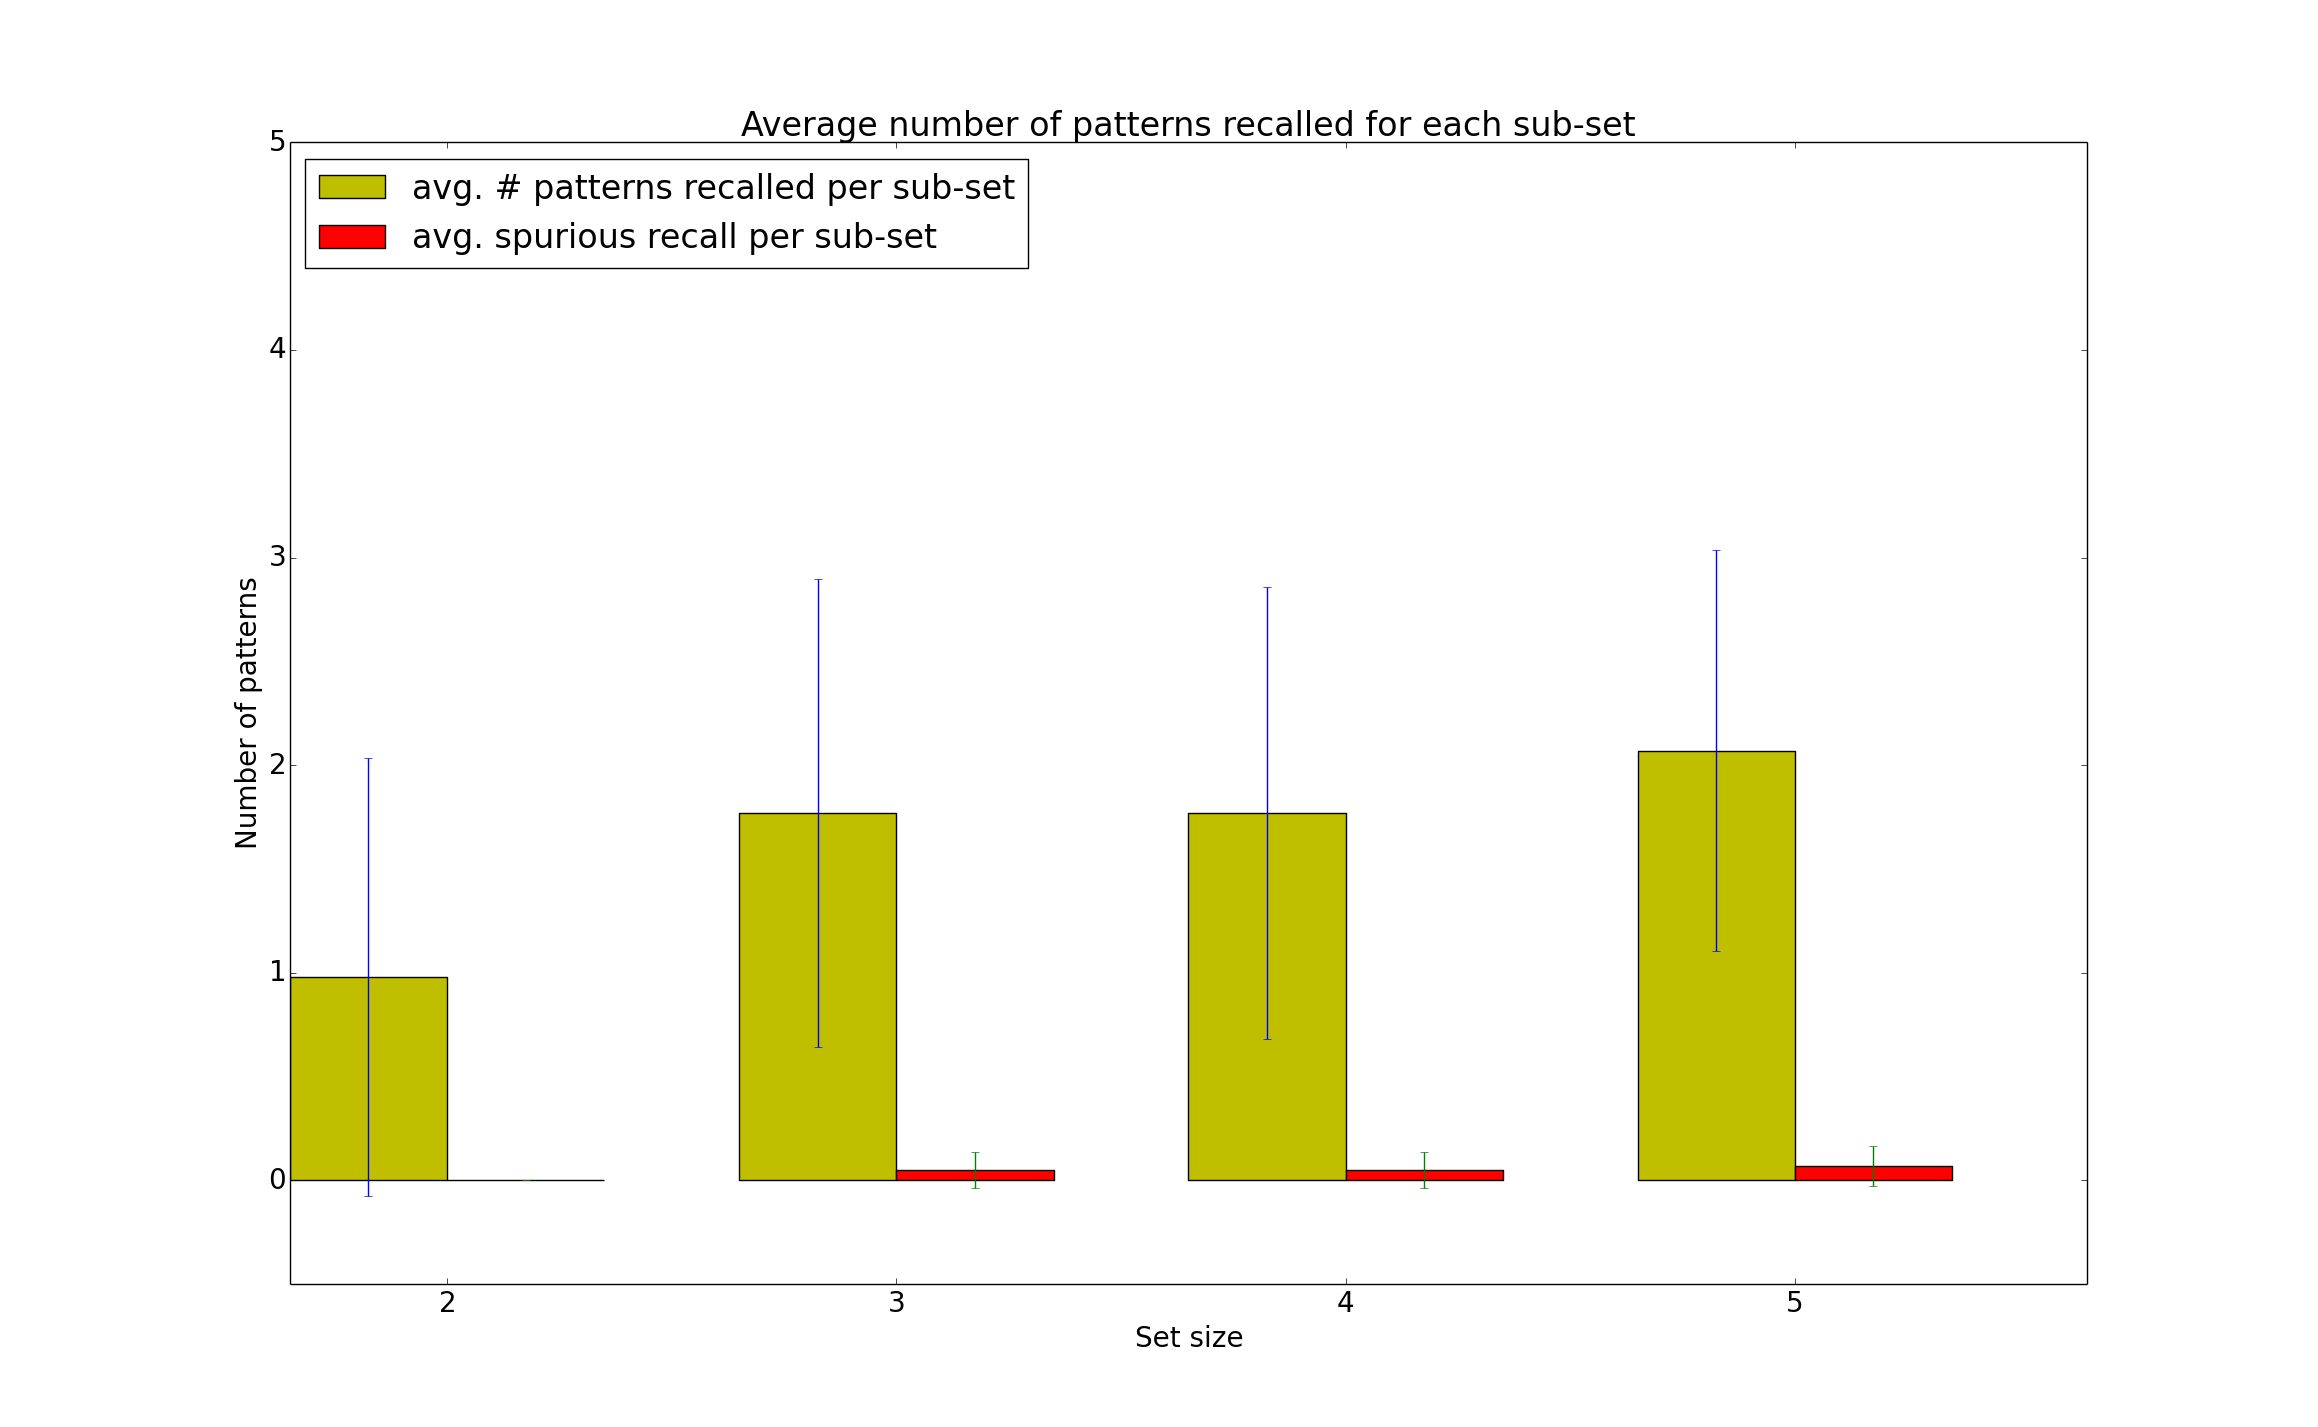
\includegraphics[width=13cm]{fig/async_false_mode_0.png}
%     \caption{async false mode 0}
%     \label{fig:async_false_mode_0}
% \end{figure}

% \begin{figure}[h!]
%     \centering
%     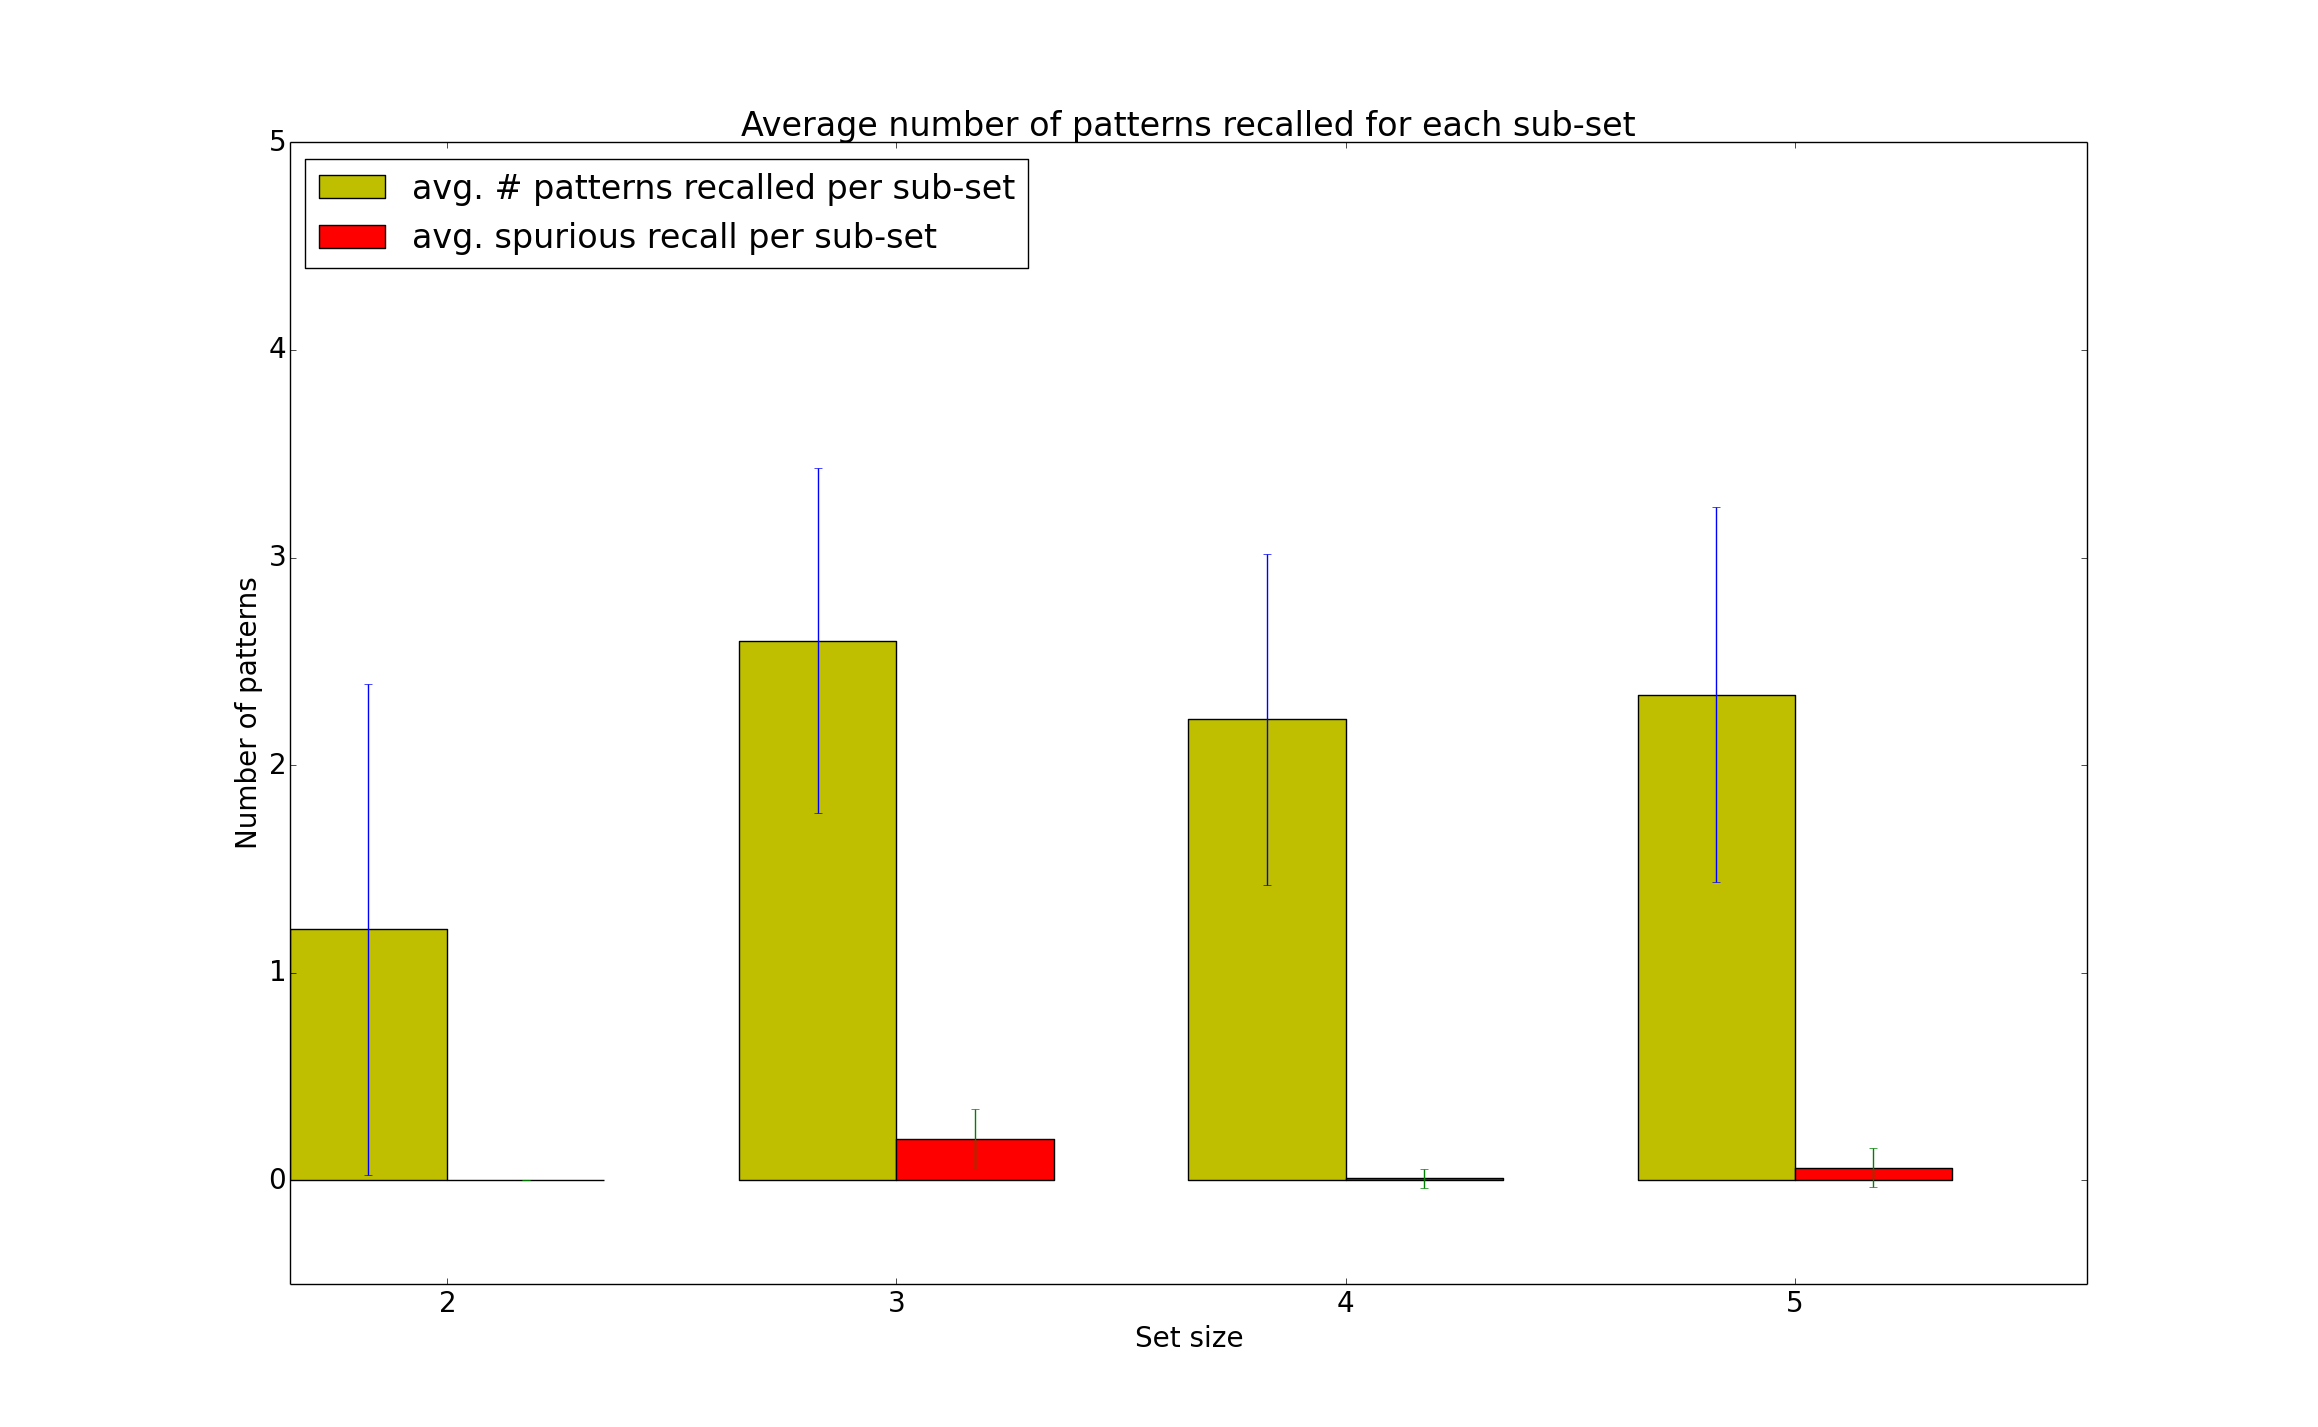
\includegraphics[width=13cm]{fig/async_false_mode_1.png}
%     \caption{async false mode 1}
%     \label{fig:async_false_mode_1}
% \end{figure}

% \subsubsection{Asynchronous updating}

% \begin{figure}[h!]
%     \centering
%     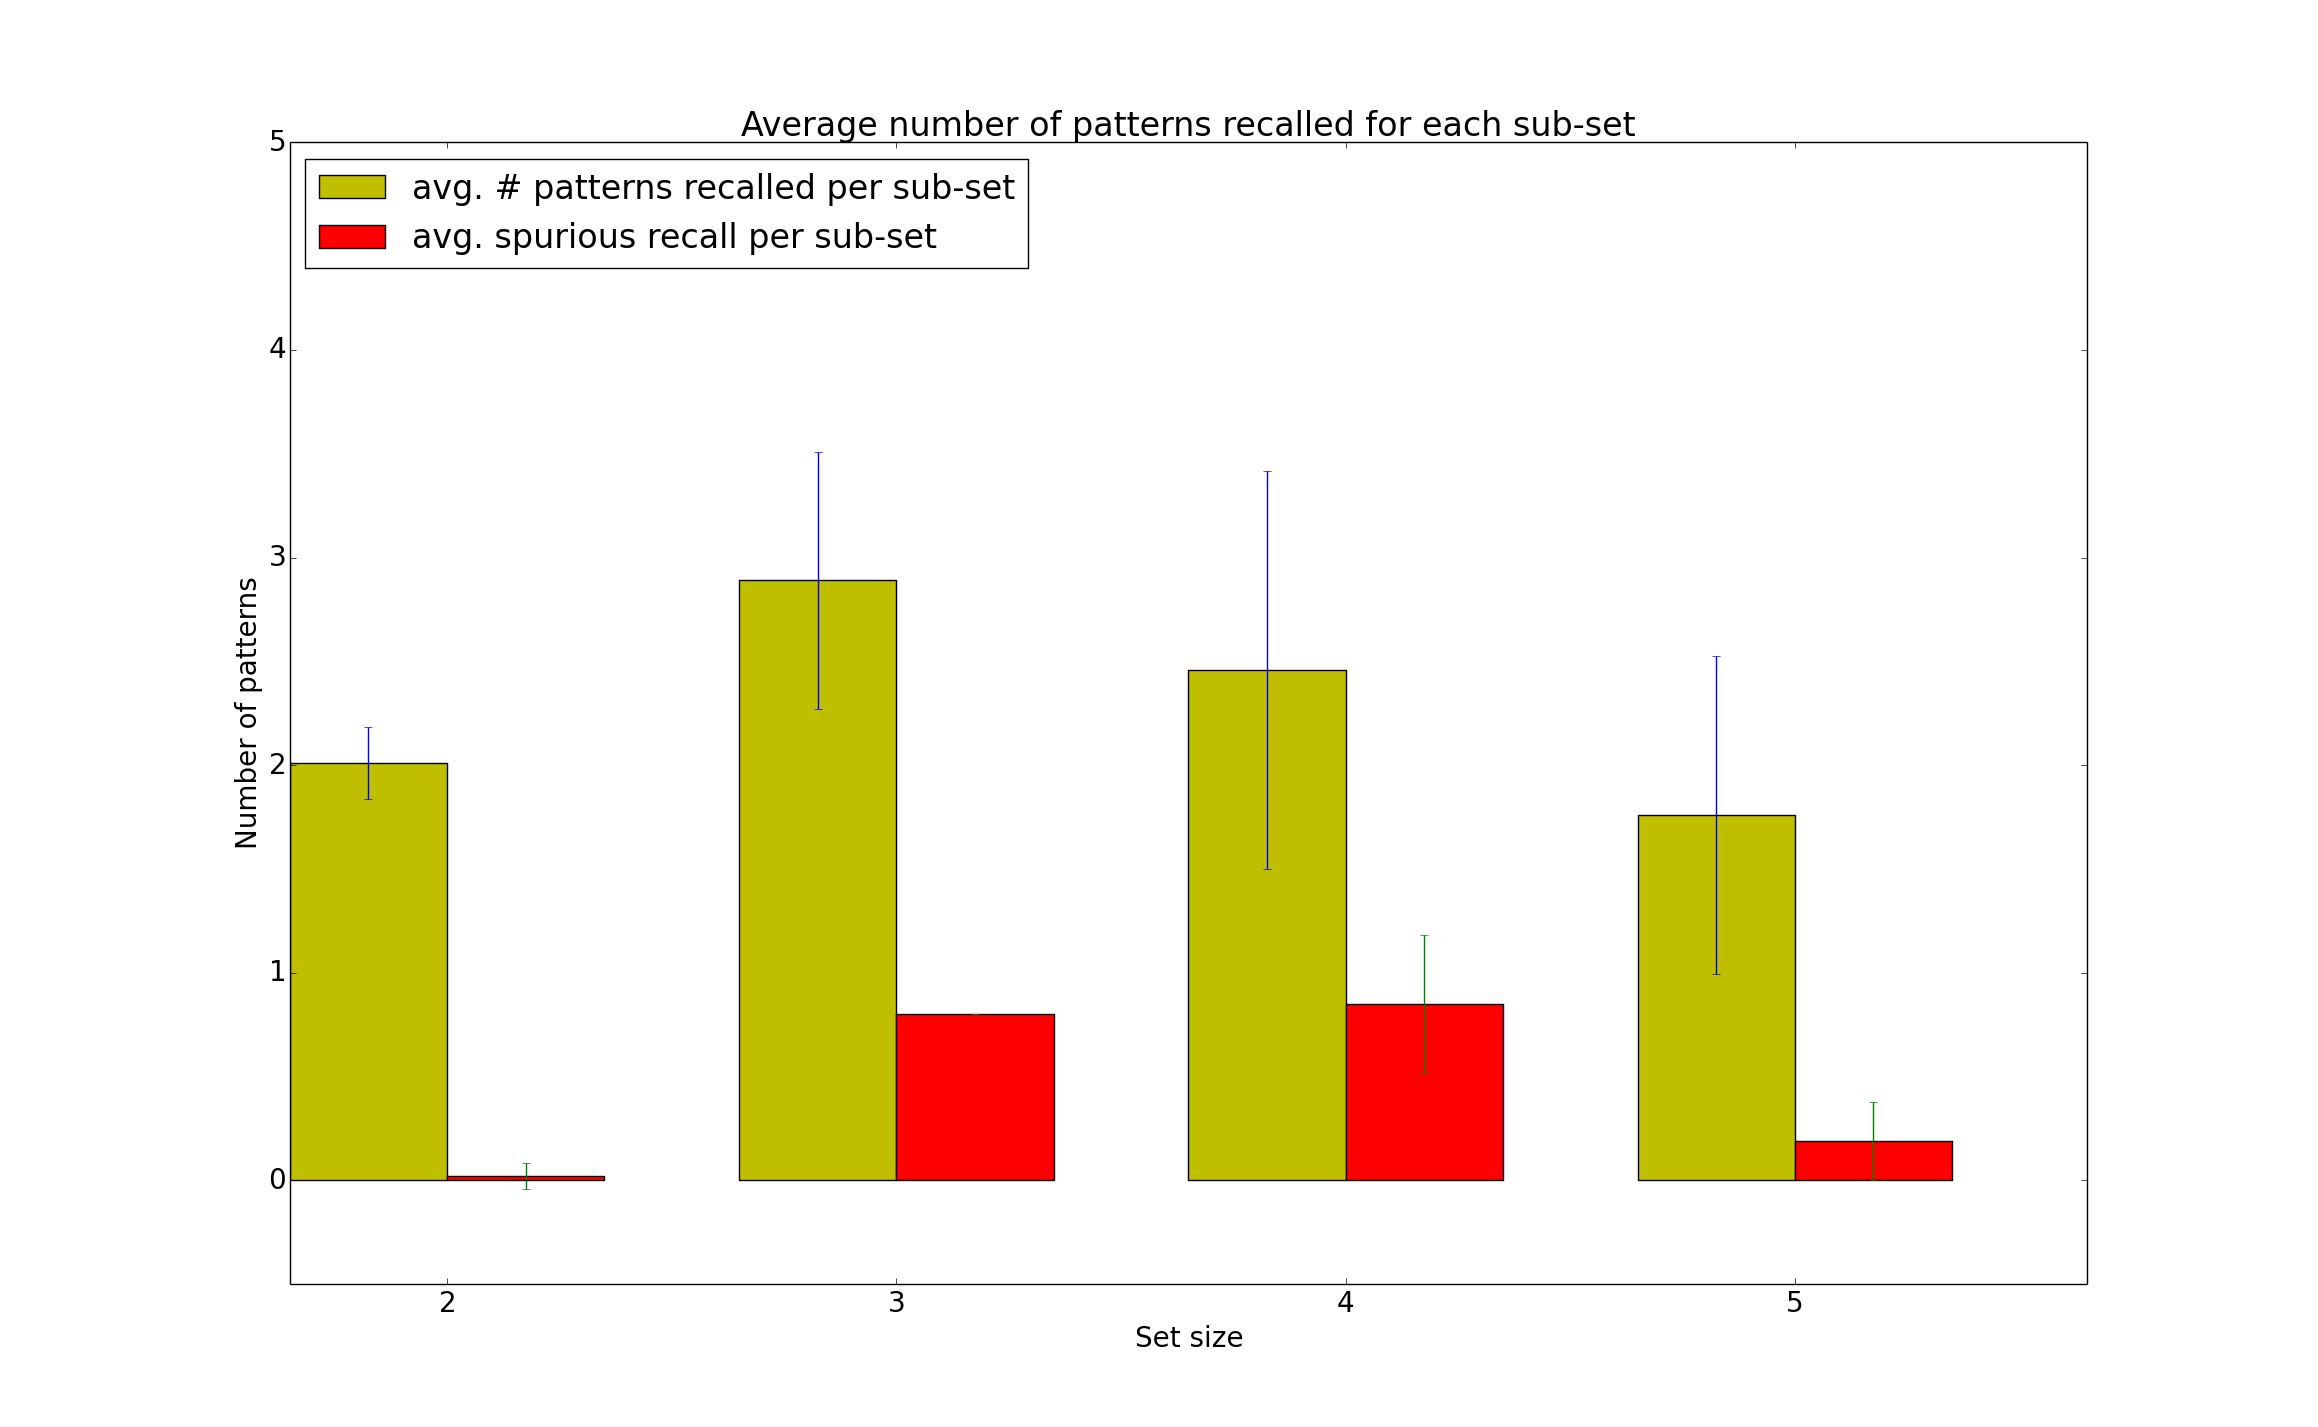
\includegraphics[width=13cm]{fig/async_true_mode_0.png}
%     \caption{async true mode 0}
%     \label{fig:async_true_mode_0}
% \end{figure}

% \begin{figure}[h!]
%     \centering
%     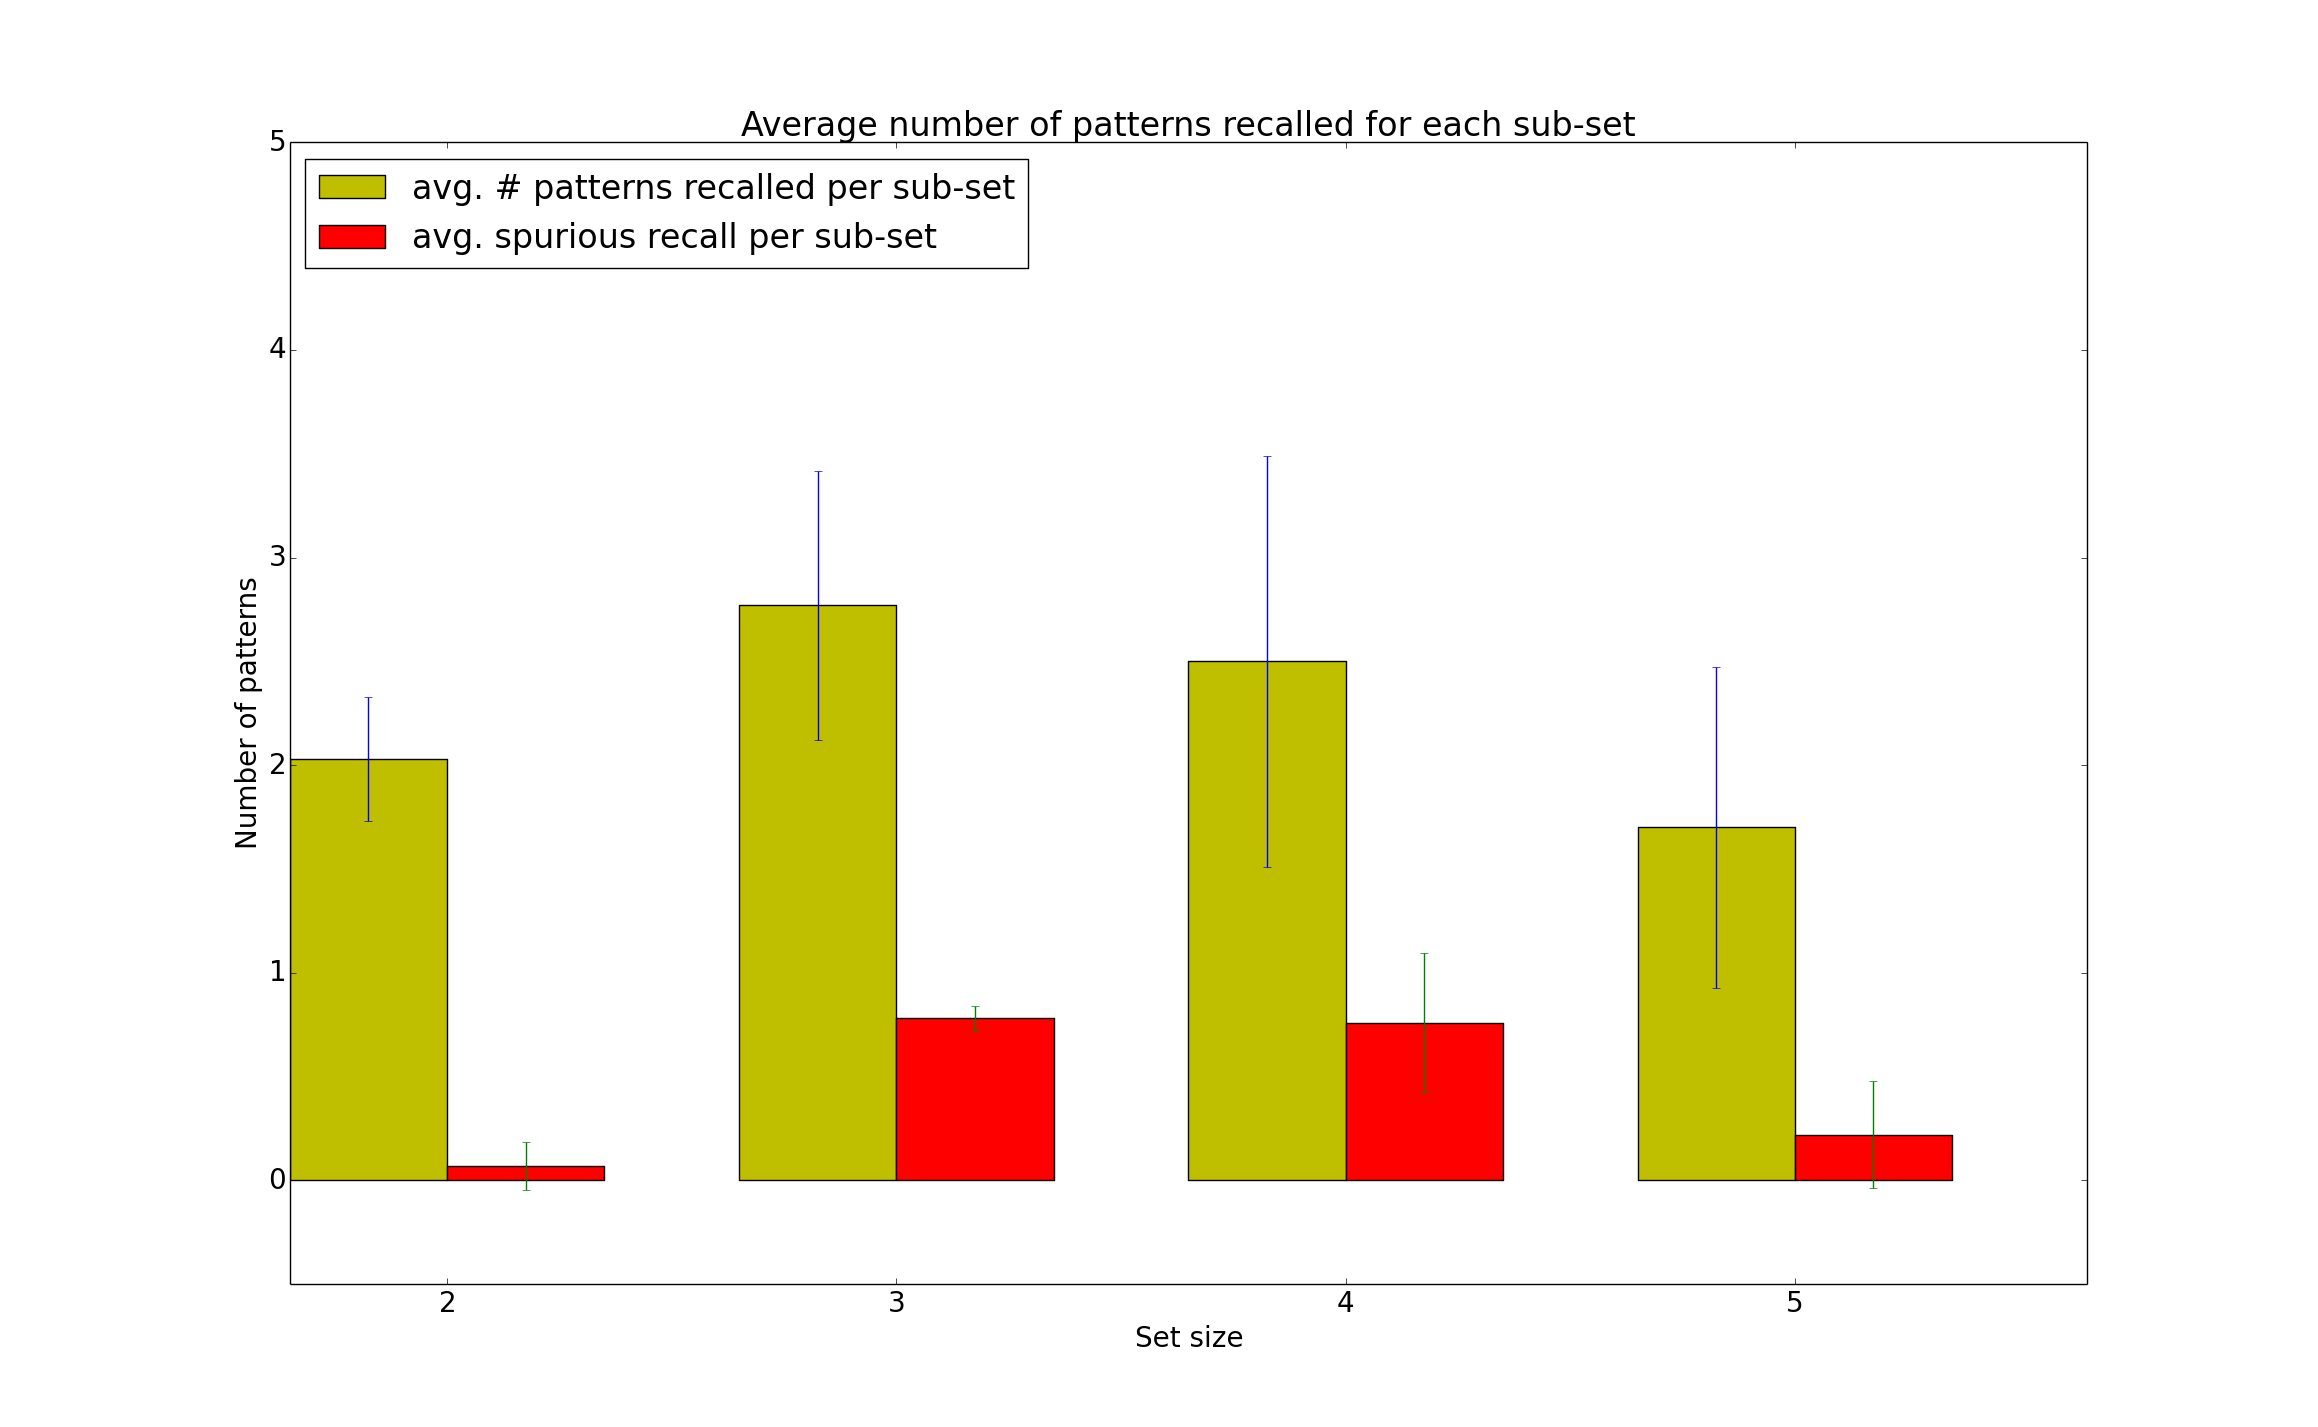
\includegraphics[width=13cm]{fig/async_true_mode_1.png}
%     \caption{async true mode 1}
%     \label{fig:async_true_mode_1}
% \end{figure}

% ========= for all ==========
\begin{figure}[h!]
    \centering
    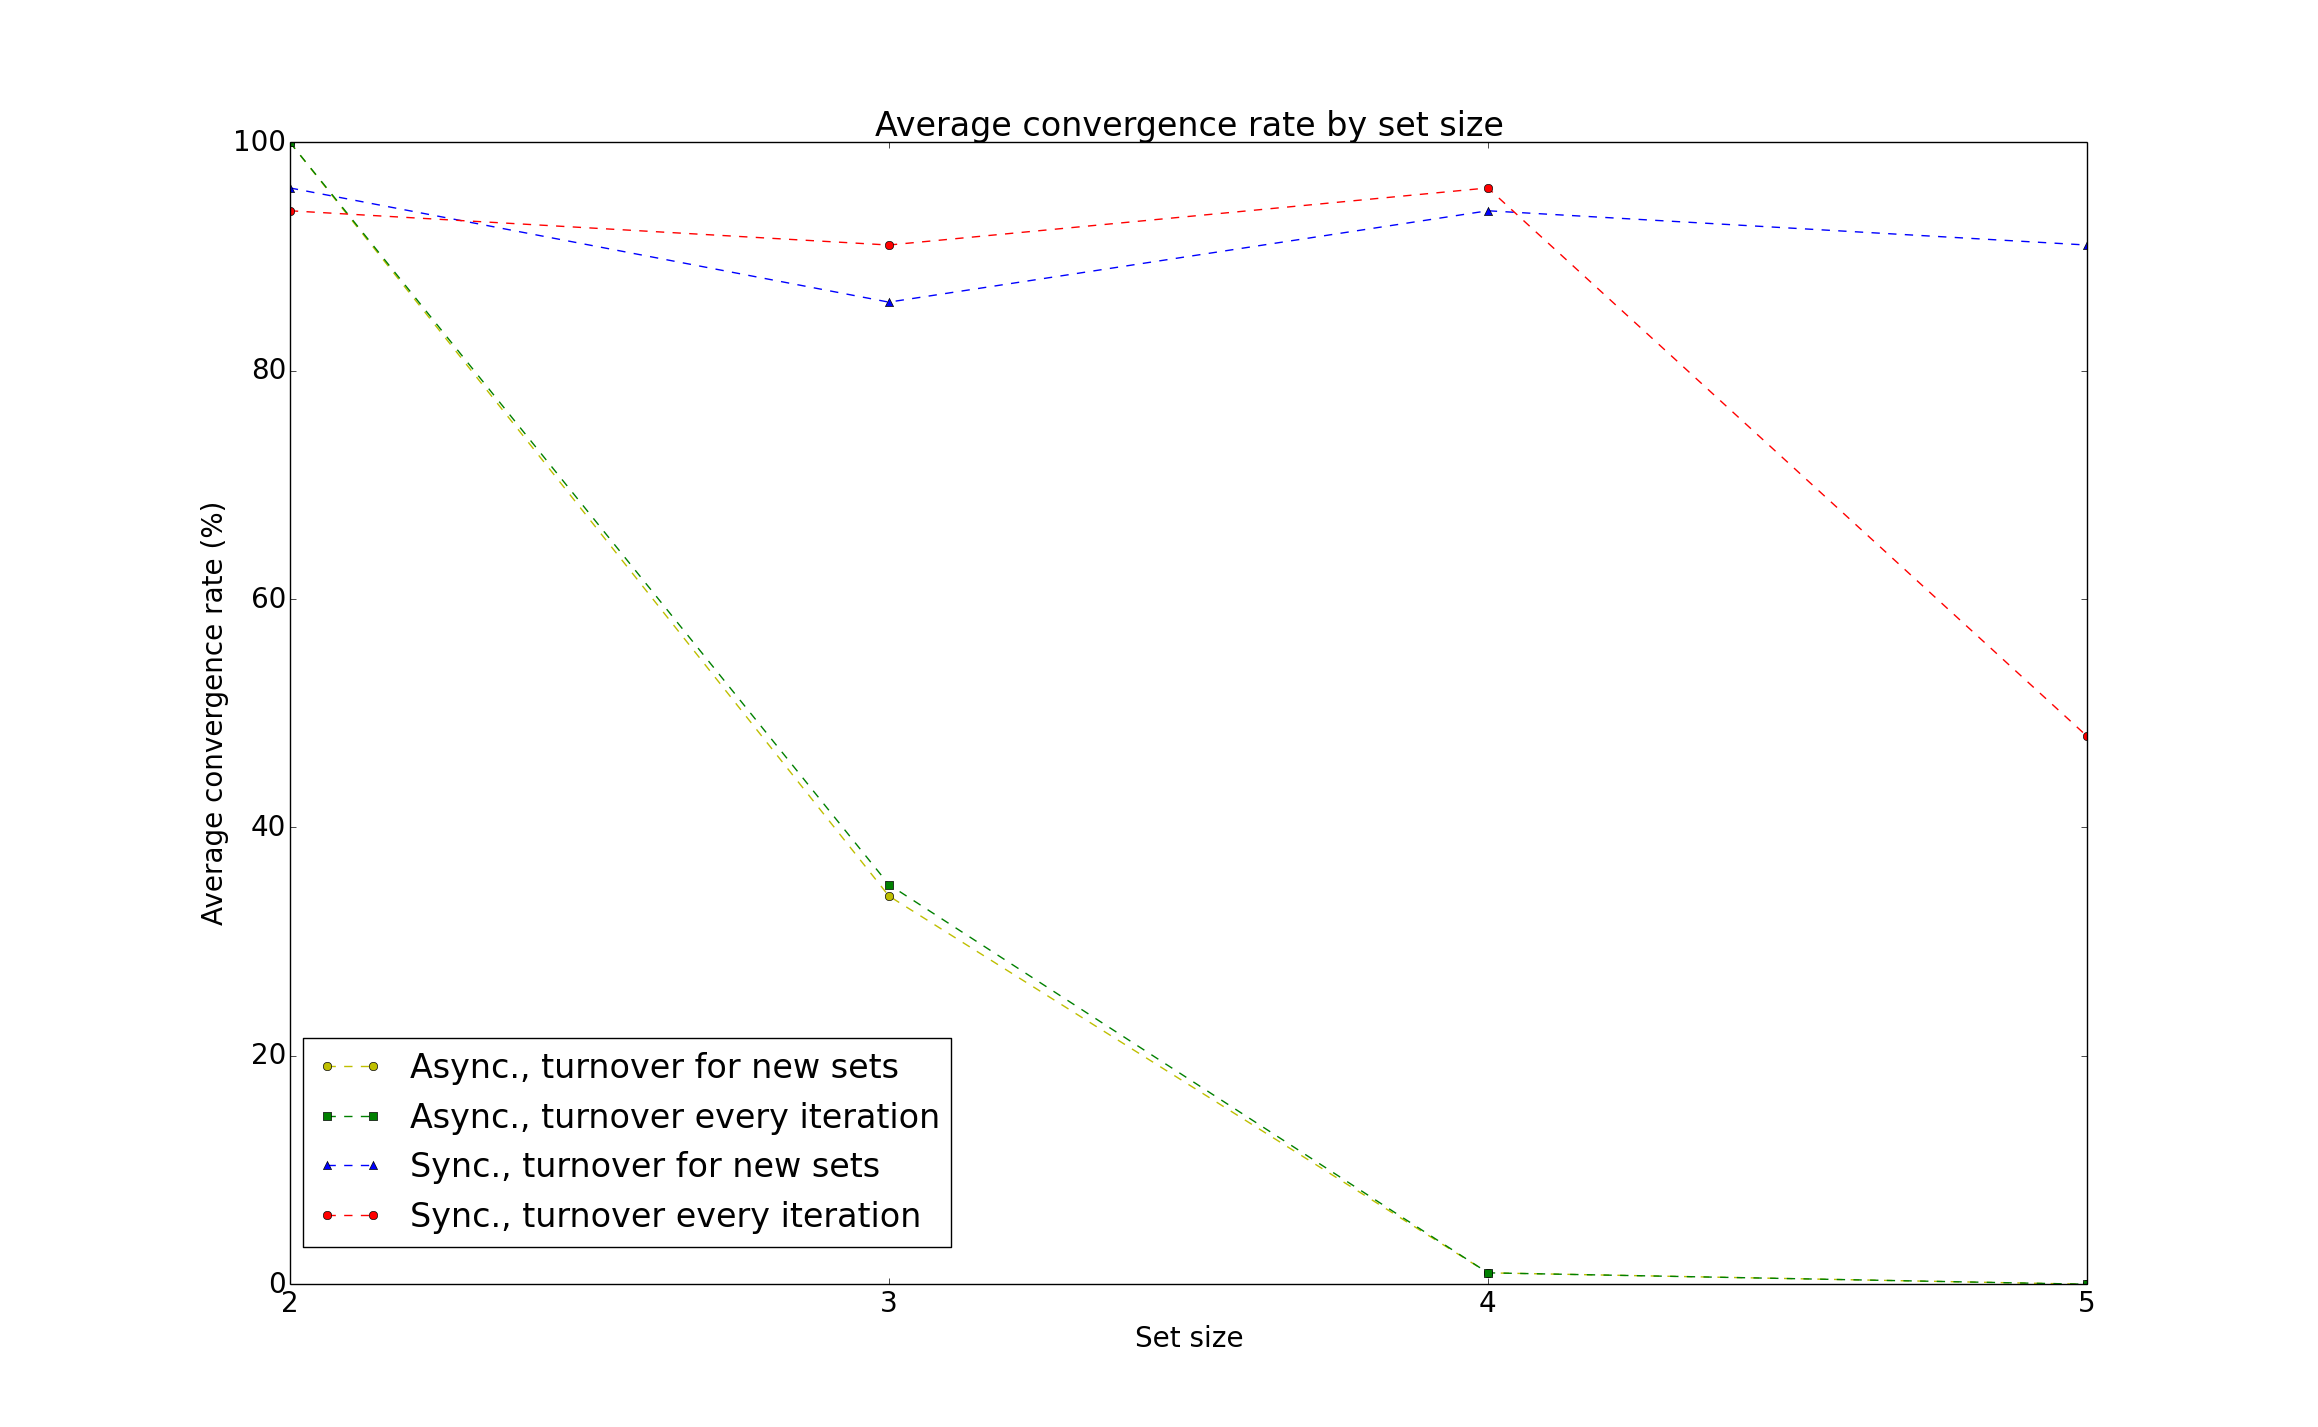
\includegraphics[width=14cm]{fig/avg_convergence_rate.png}
    \caption{avg convergence by set size, dentate gyrus weighting 25, turnover rate $0.5$.}
    \label{fig:avg_convergence_rate}
\end{figure}

\begin{figure}[h!]
    \centering
    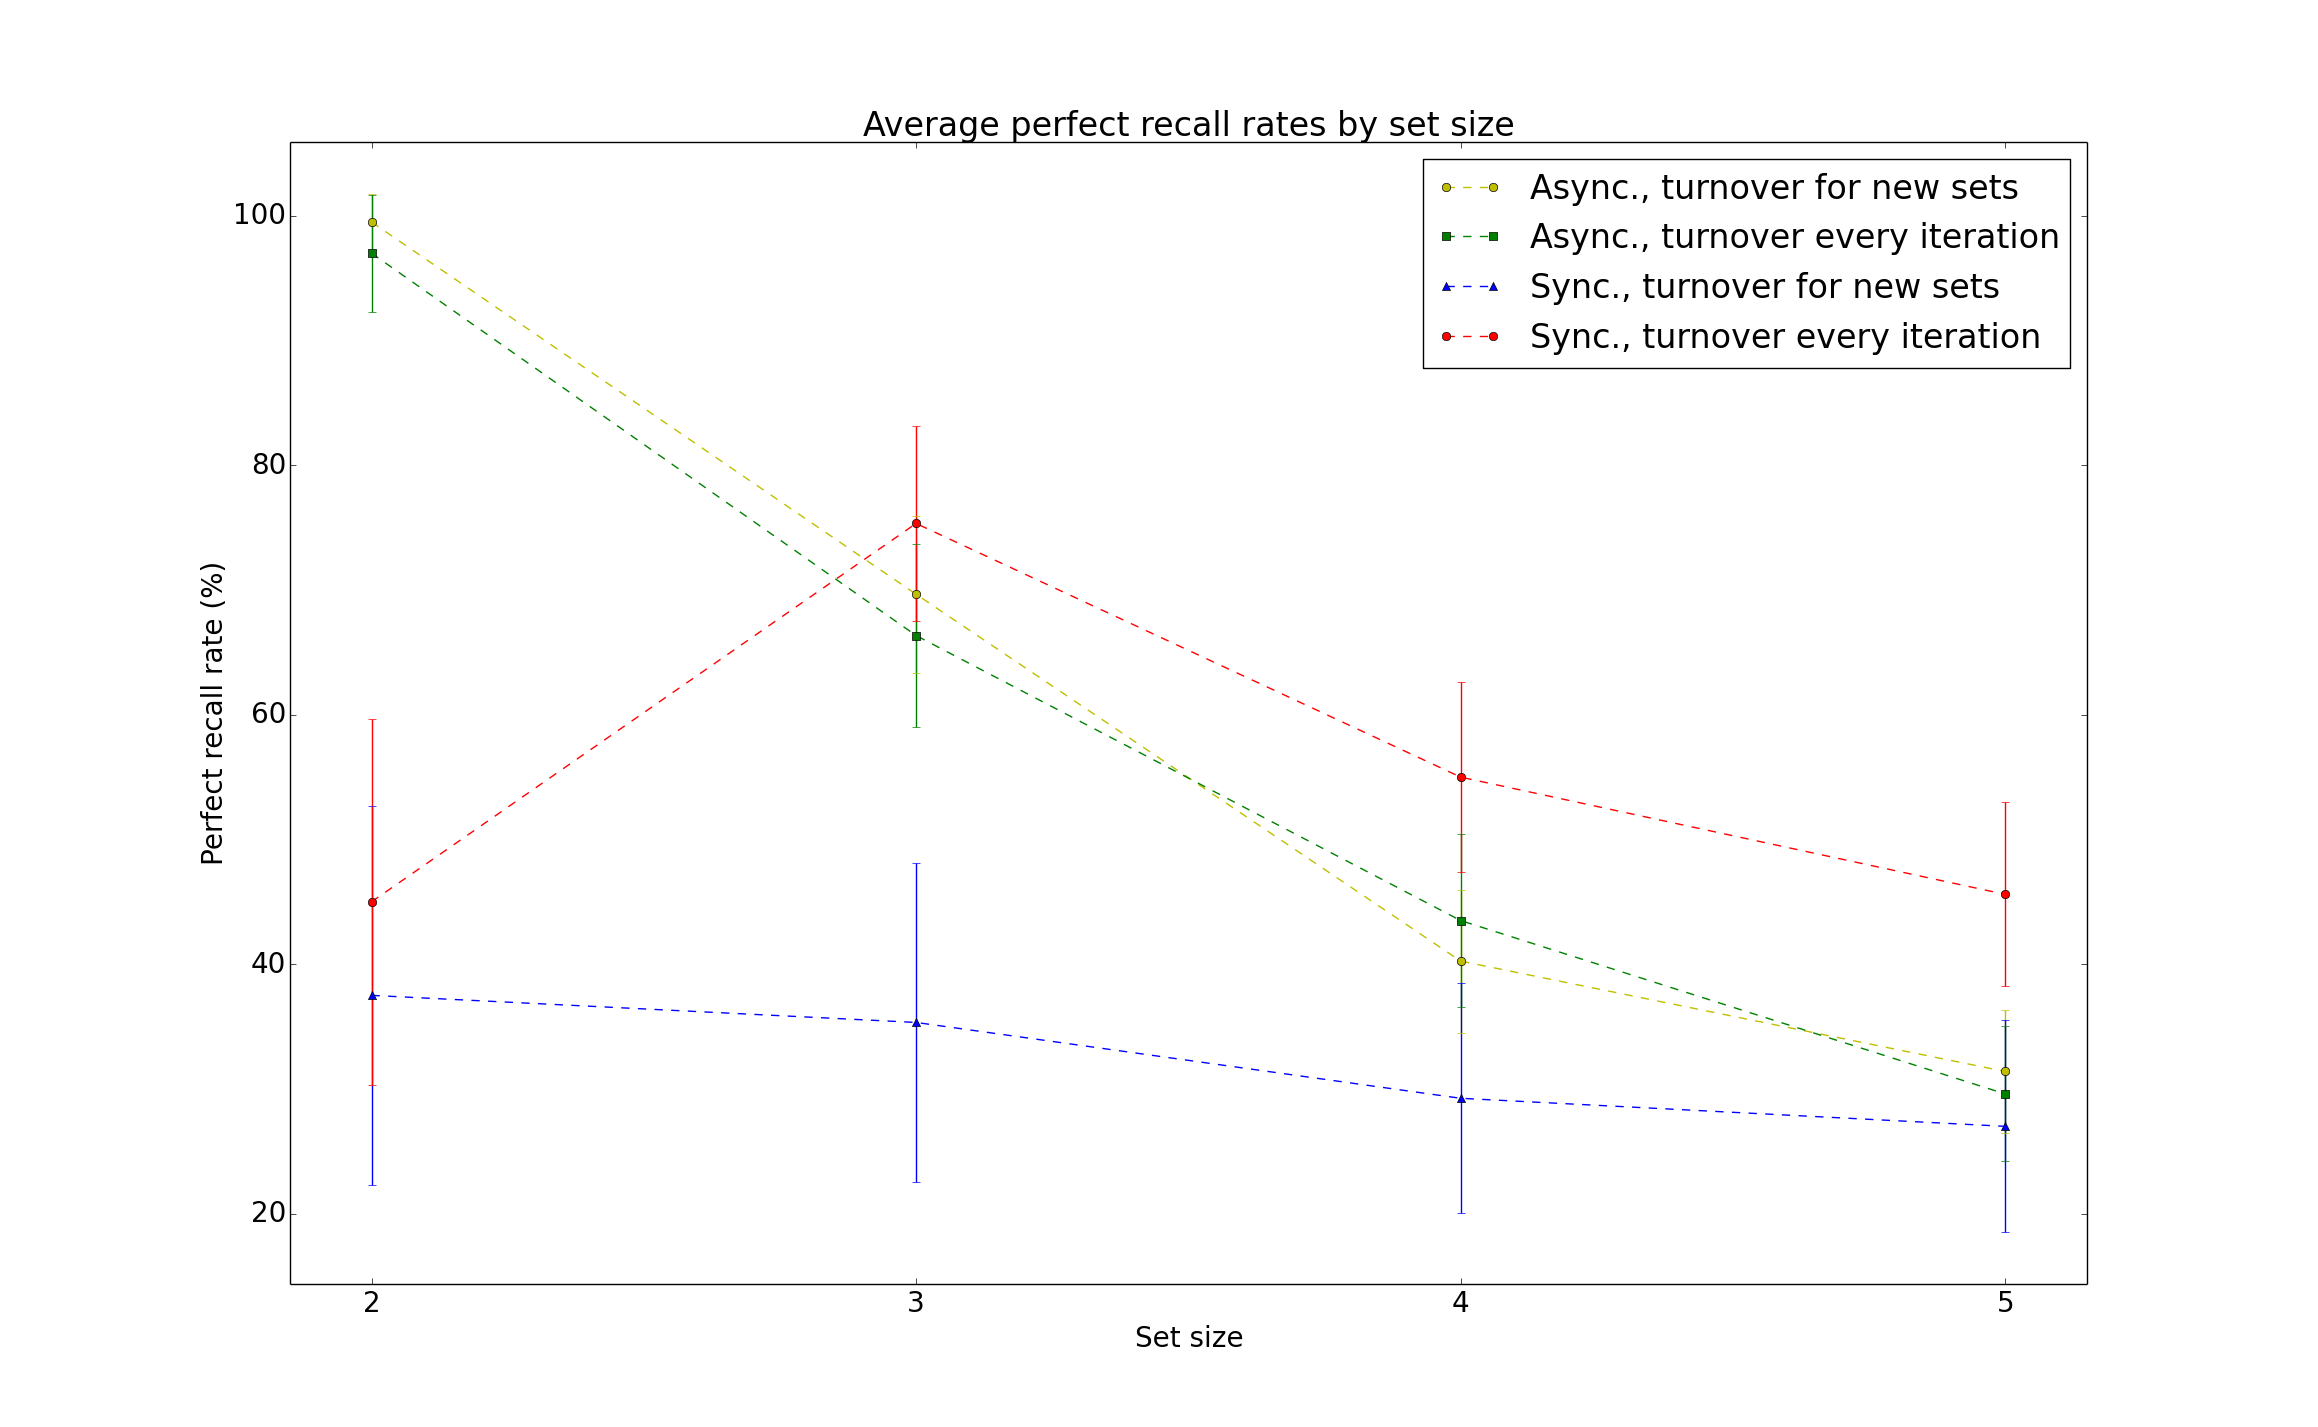
\includegraphics[width=14cm]{fig/avg_perfect_recall_rates.png}
    \caption{perf recall by set size, dentate gyrus weighting 25, turnover rate $0.5$.}
    \label{fig:avg_perfect_recall_rates}
\end{figure}

\begin{figure}[h!]
    \centering
    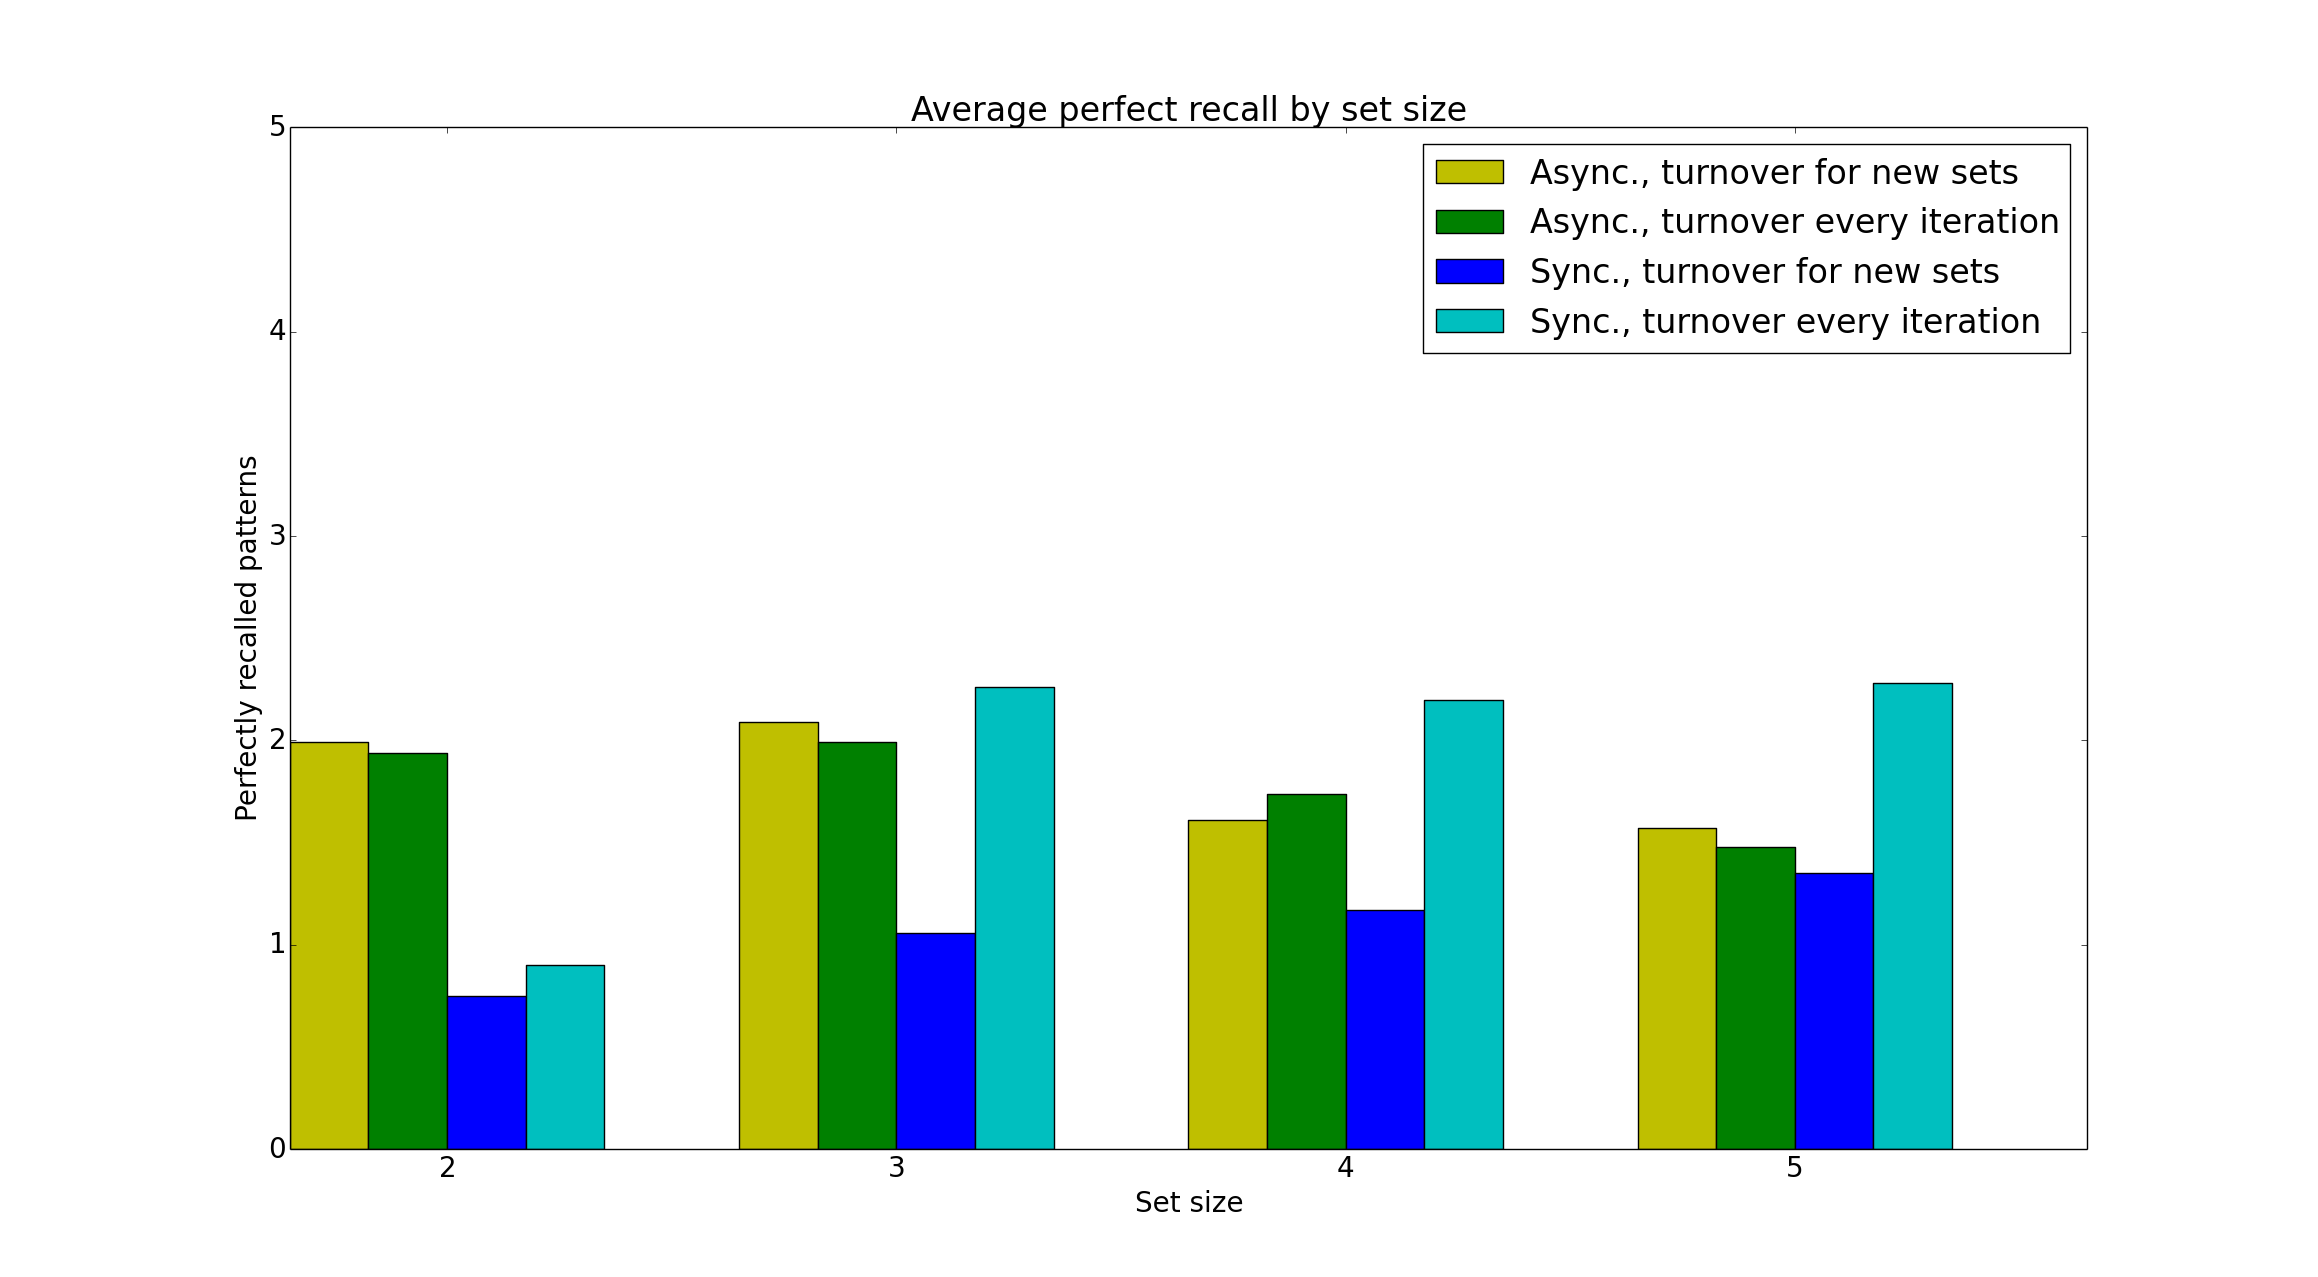
\includegraphics[width=14cm]{fig/average_perfect_recall_rates_by_set_size_bars_reset_for_every_experiment}
    \caption{perf recall by set size bars, dentate gyrus weighting 25, turnover rate $0.5$.}
    \label{fig:avg_perfect_recall_bars}
\end{figure}

\begin{figure}[h!]
    \centering
    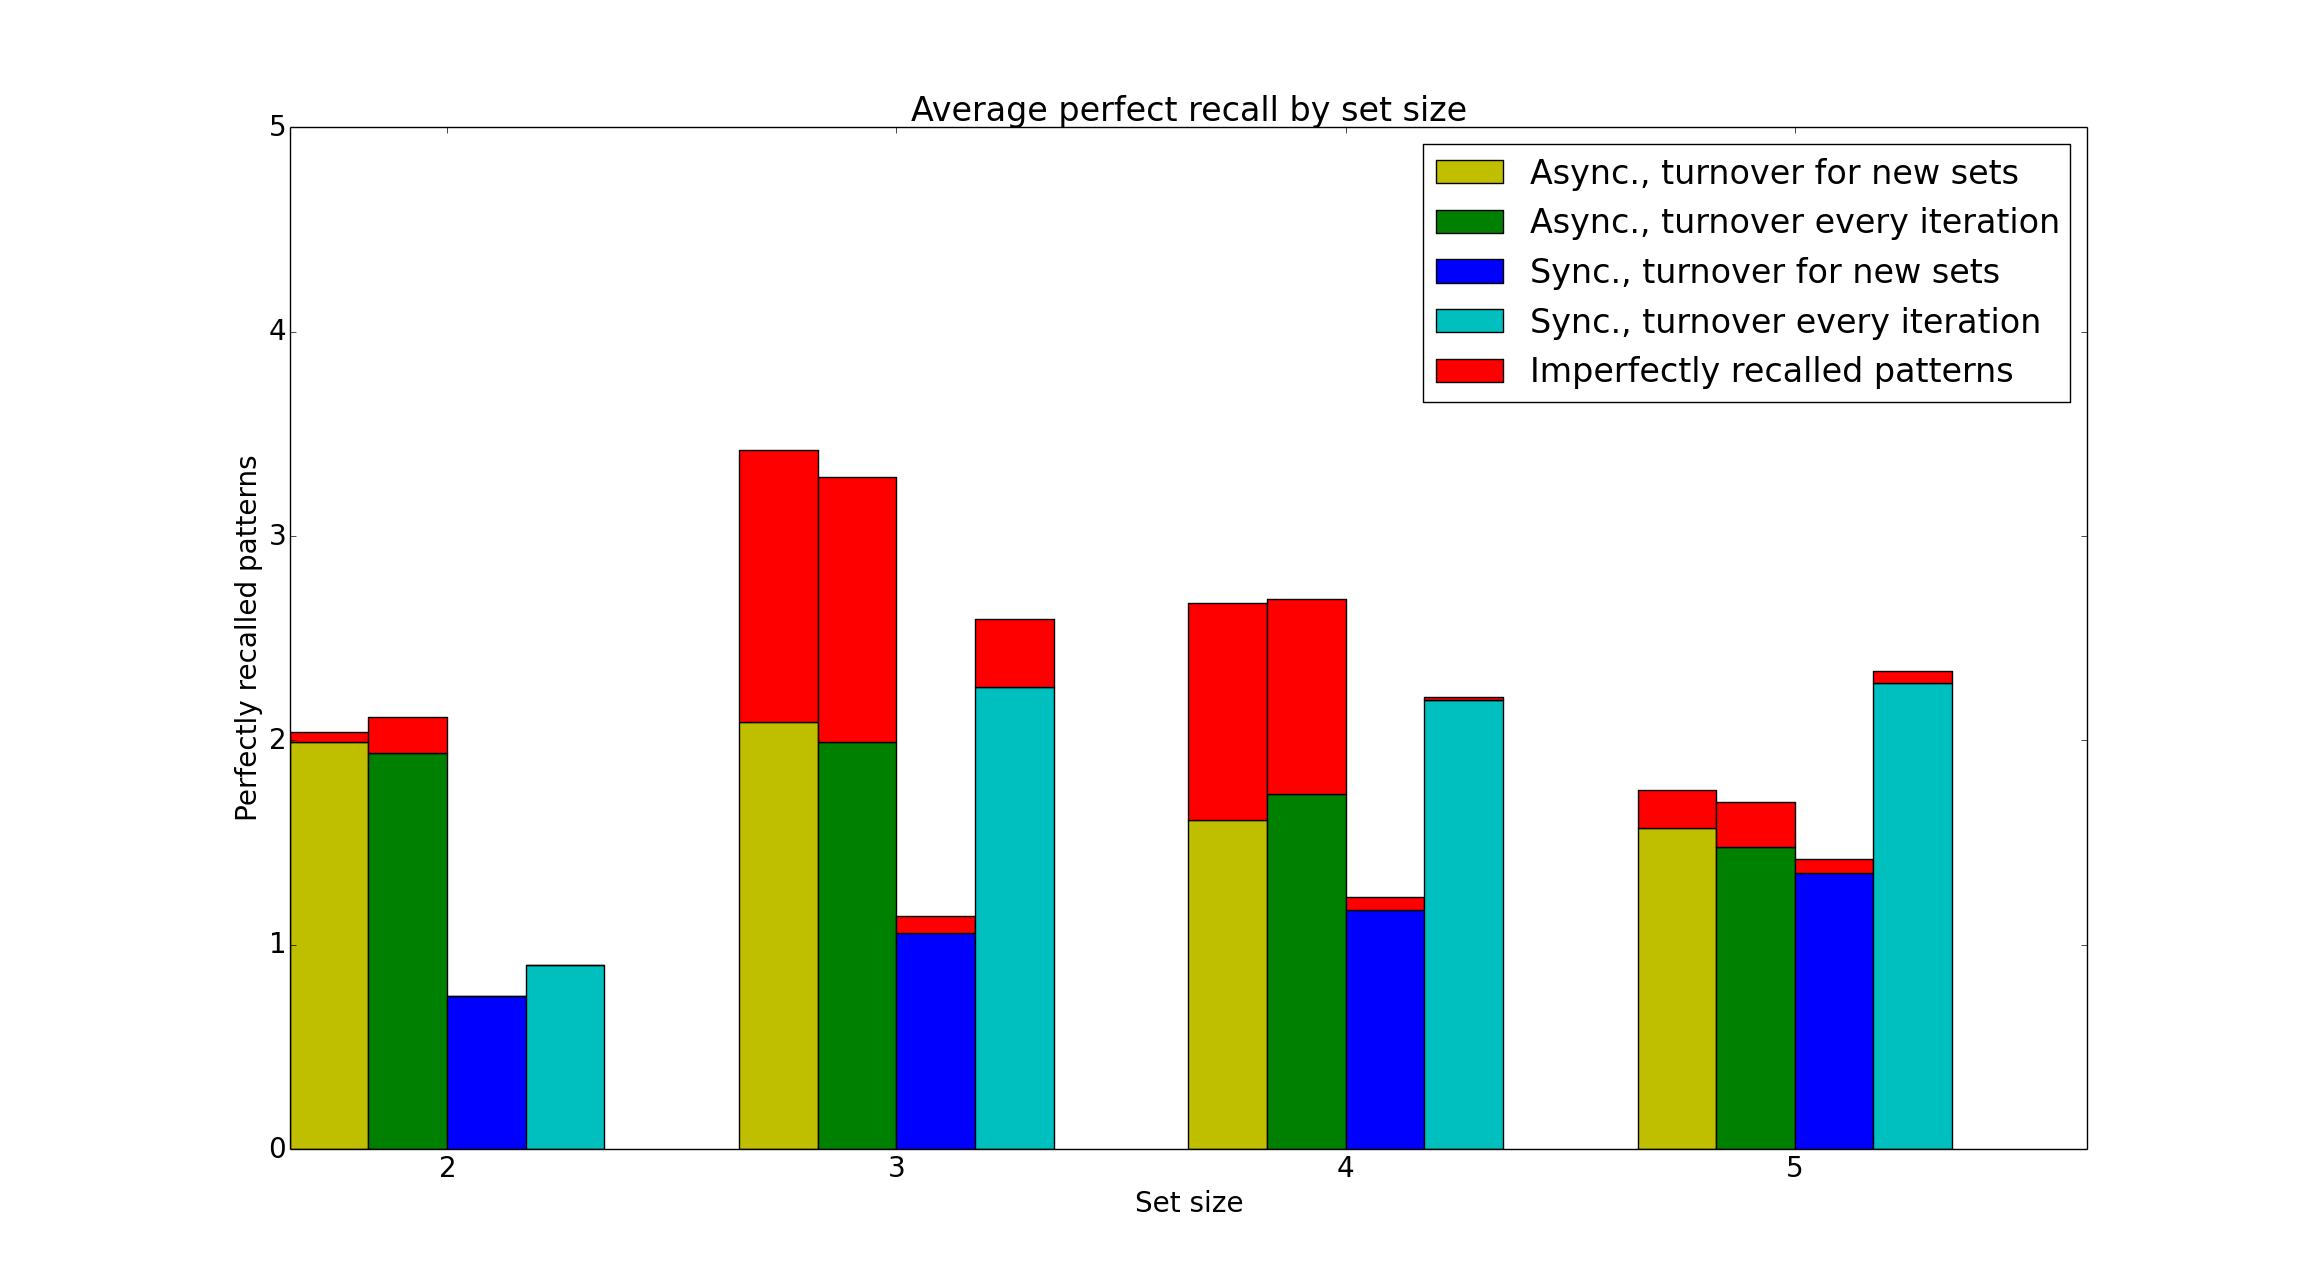
\includegraphics[width=14cm]{fig/average_perfect_recall_rates_by_set_size_bars_reset_for_every_experiment_with_imperfectly_recalled_patterns.png}
    \caption{perf recall by set size bars with spurious, dentate gyrus weighting 25, turnover rate $0.5$.}
    \label{fig:avg_perfect_recall_rates_with_spurious_bars}
\end{figure}

% \begin{figure}[h!]
%     \centering
%     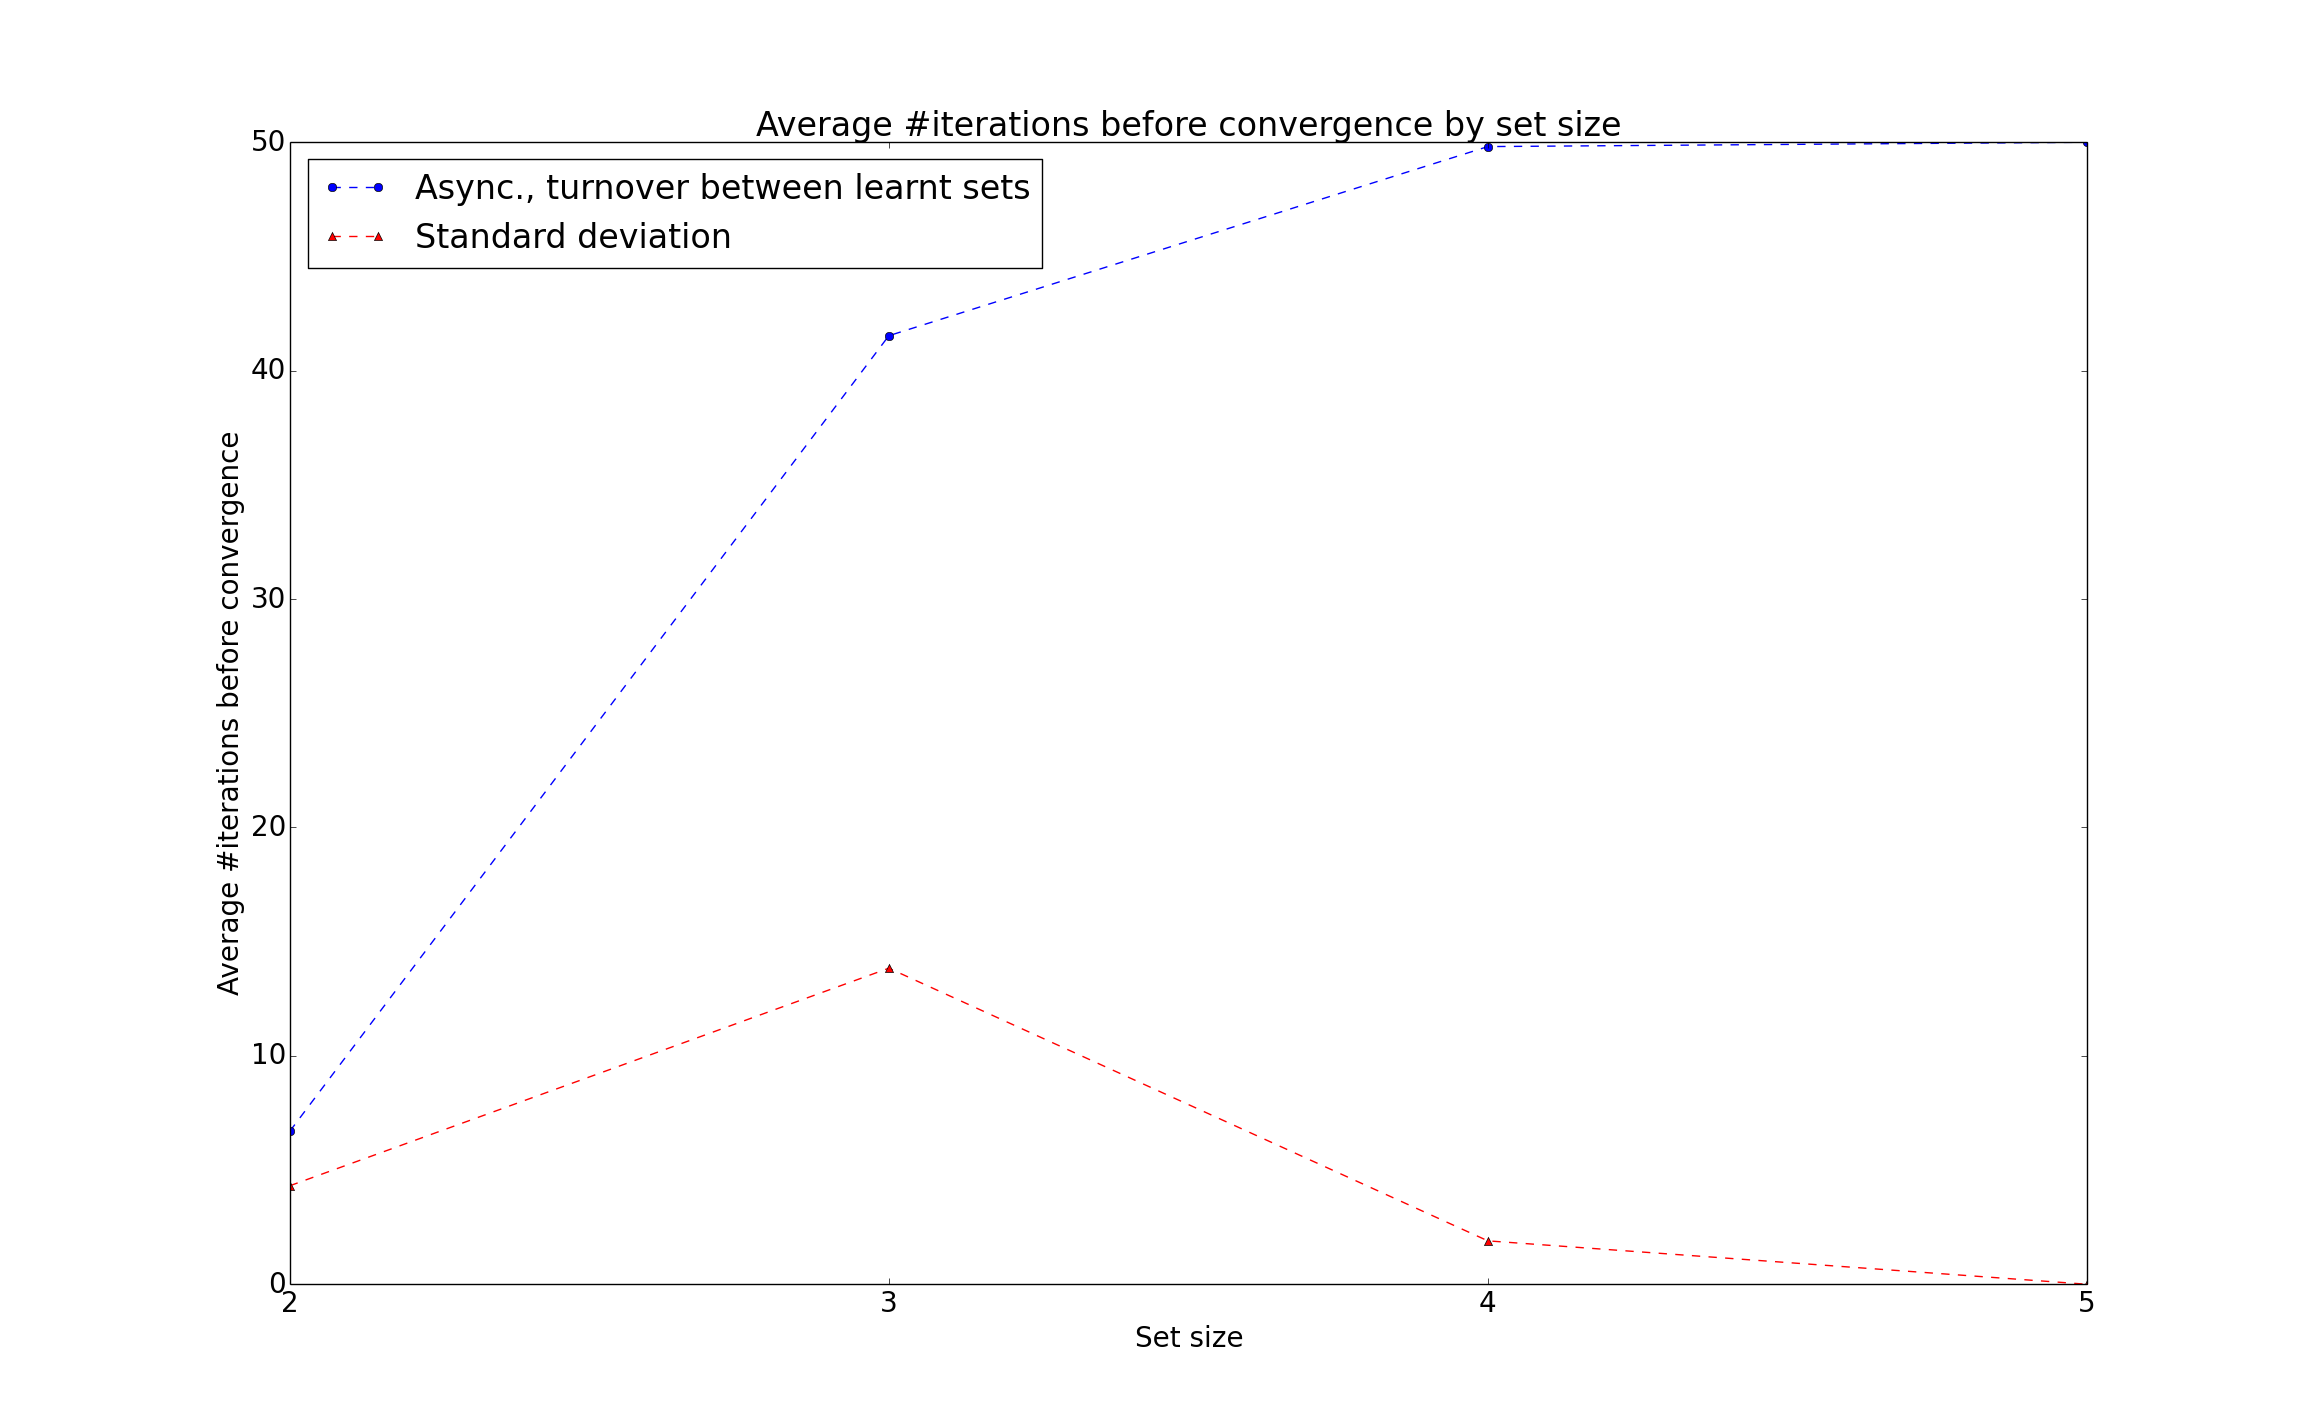
\includegraphics[width=13cm]{fig/avg_convergence_iterations_async_true_mode_0.png}
%     \caption{avg iters to convergence, most successful; async true mode 0}
%     \label{fig:avg_convergence_iterations_async_true_mode_0}
% \end{figure}

% \begin{figure}[h!]
%     \centering
%     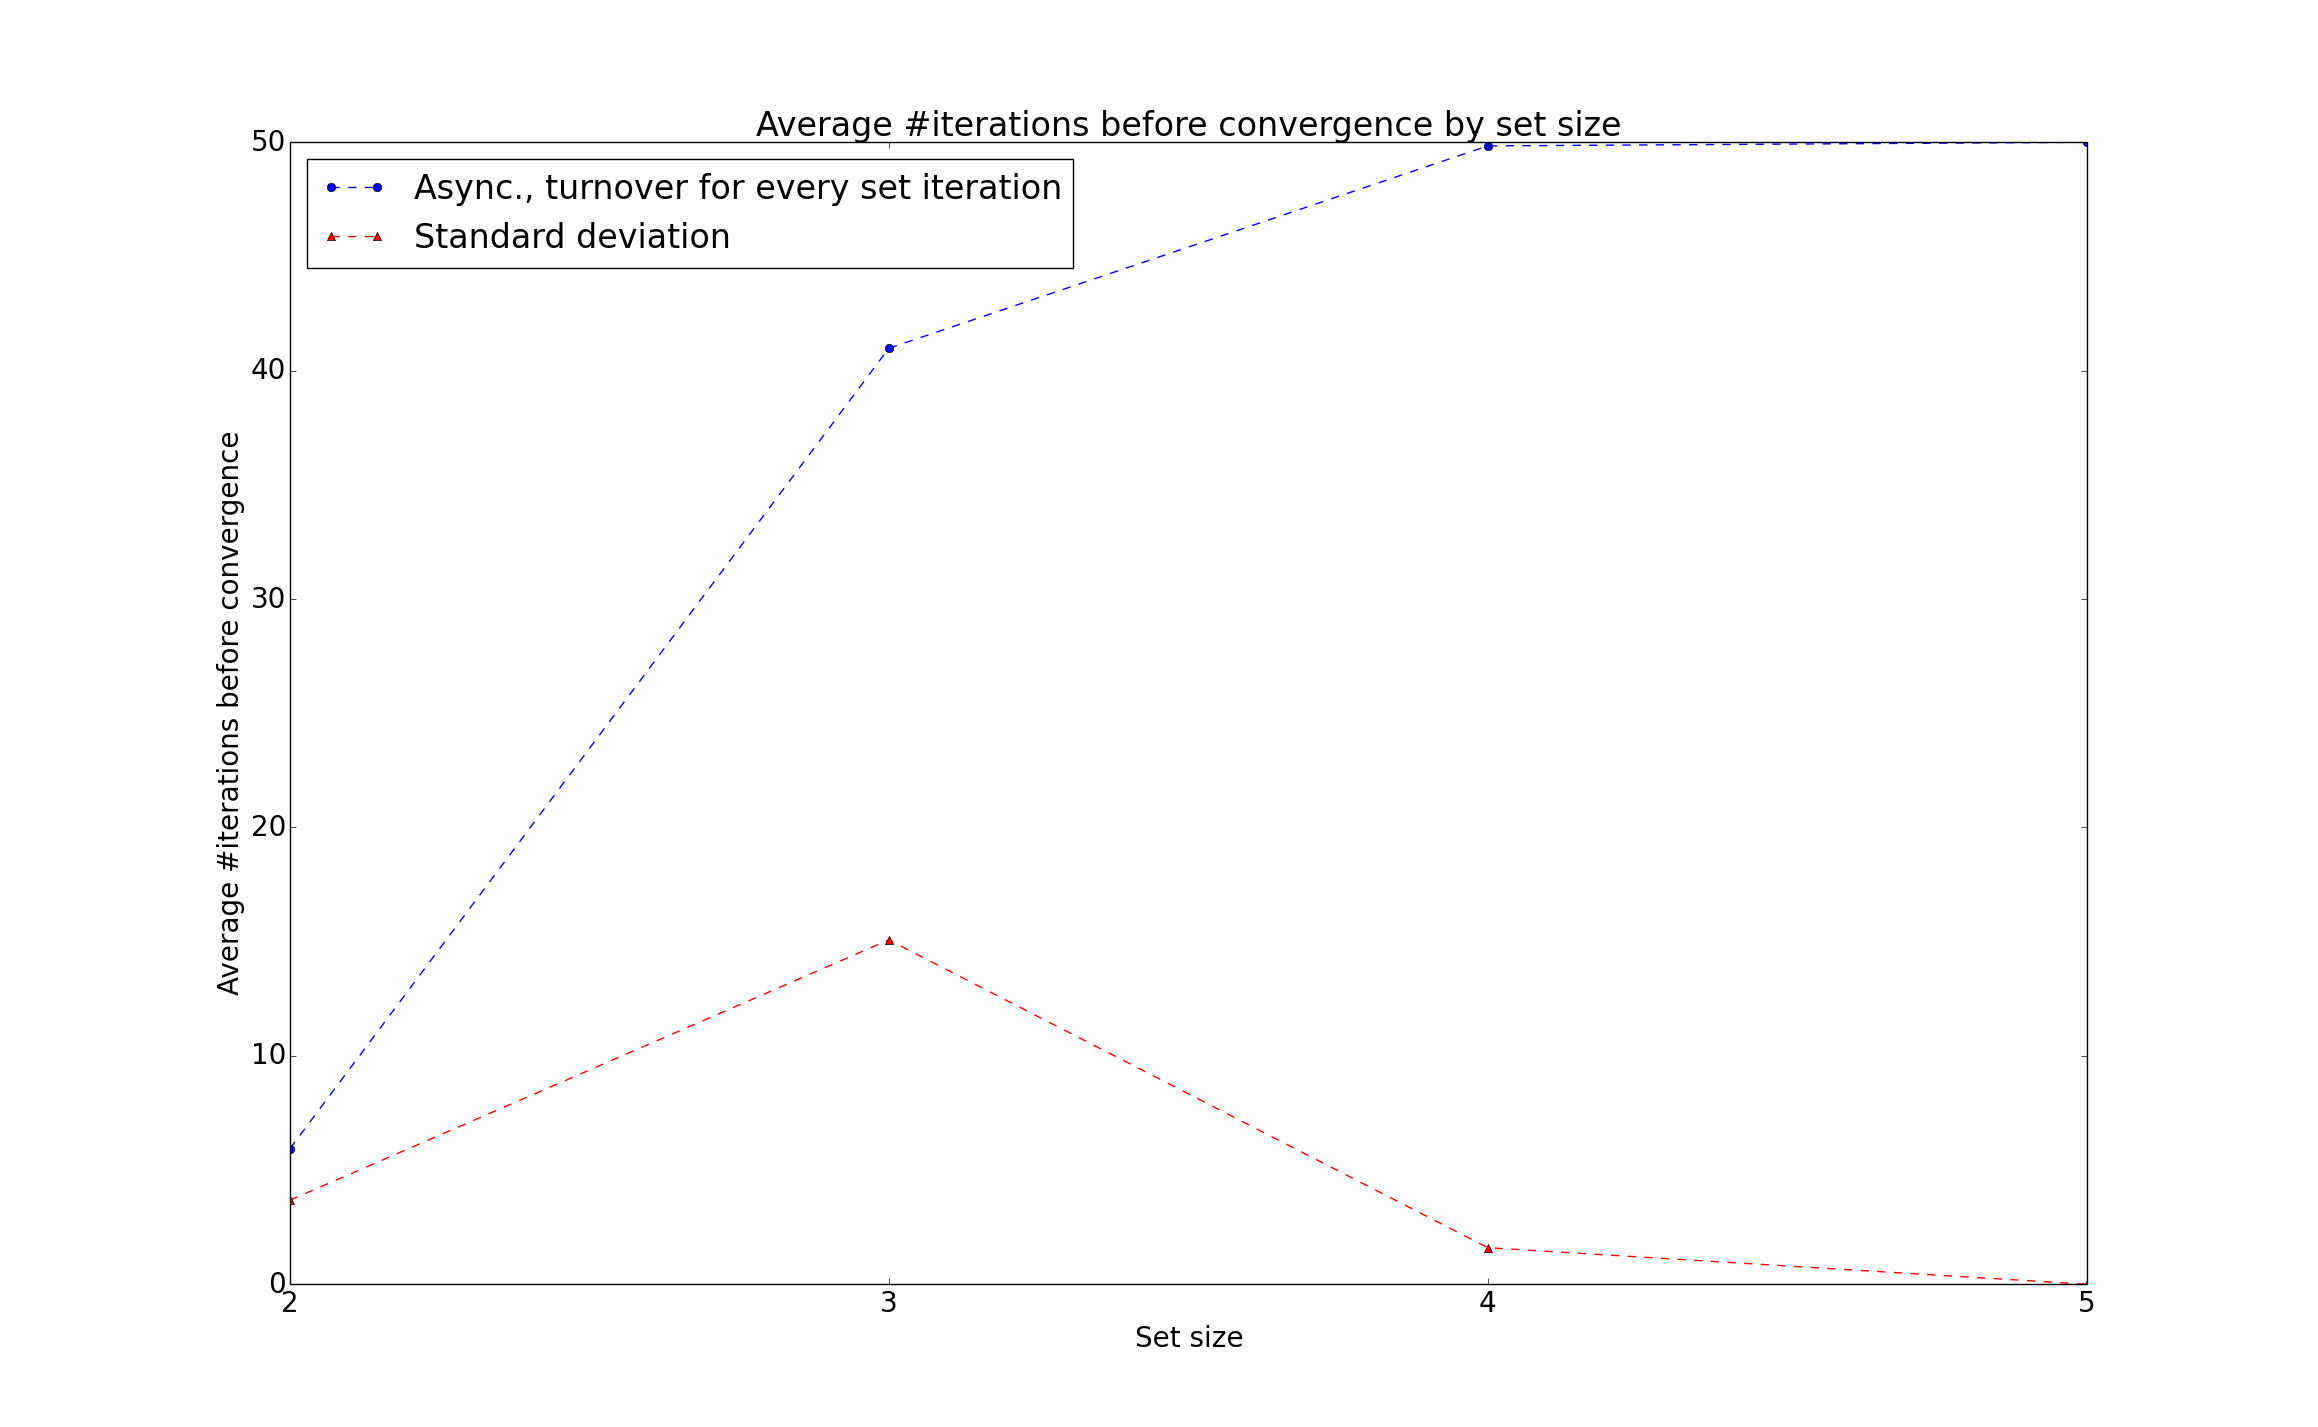
\includegraphics[width=13cm]{fig/avg_convergence_iterations_async_true_mode_1.png}
%     \caption{avg iters to convergence, most successful; async true mode 1}
%     \label{fig:avg_convergence_iterations_async_true_mode_1}
% \end{figure}

% \begin{figure}[h!]
%     \centering
%     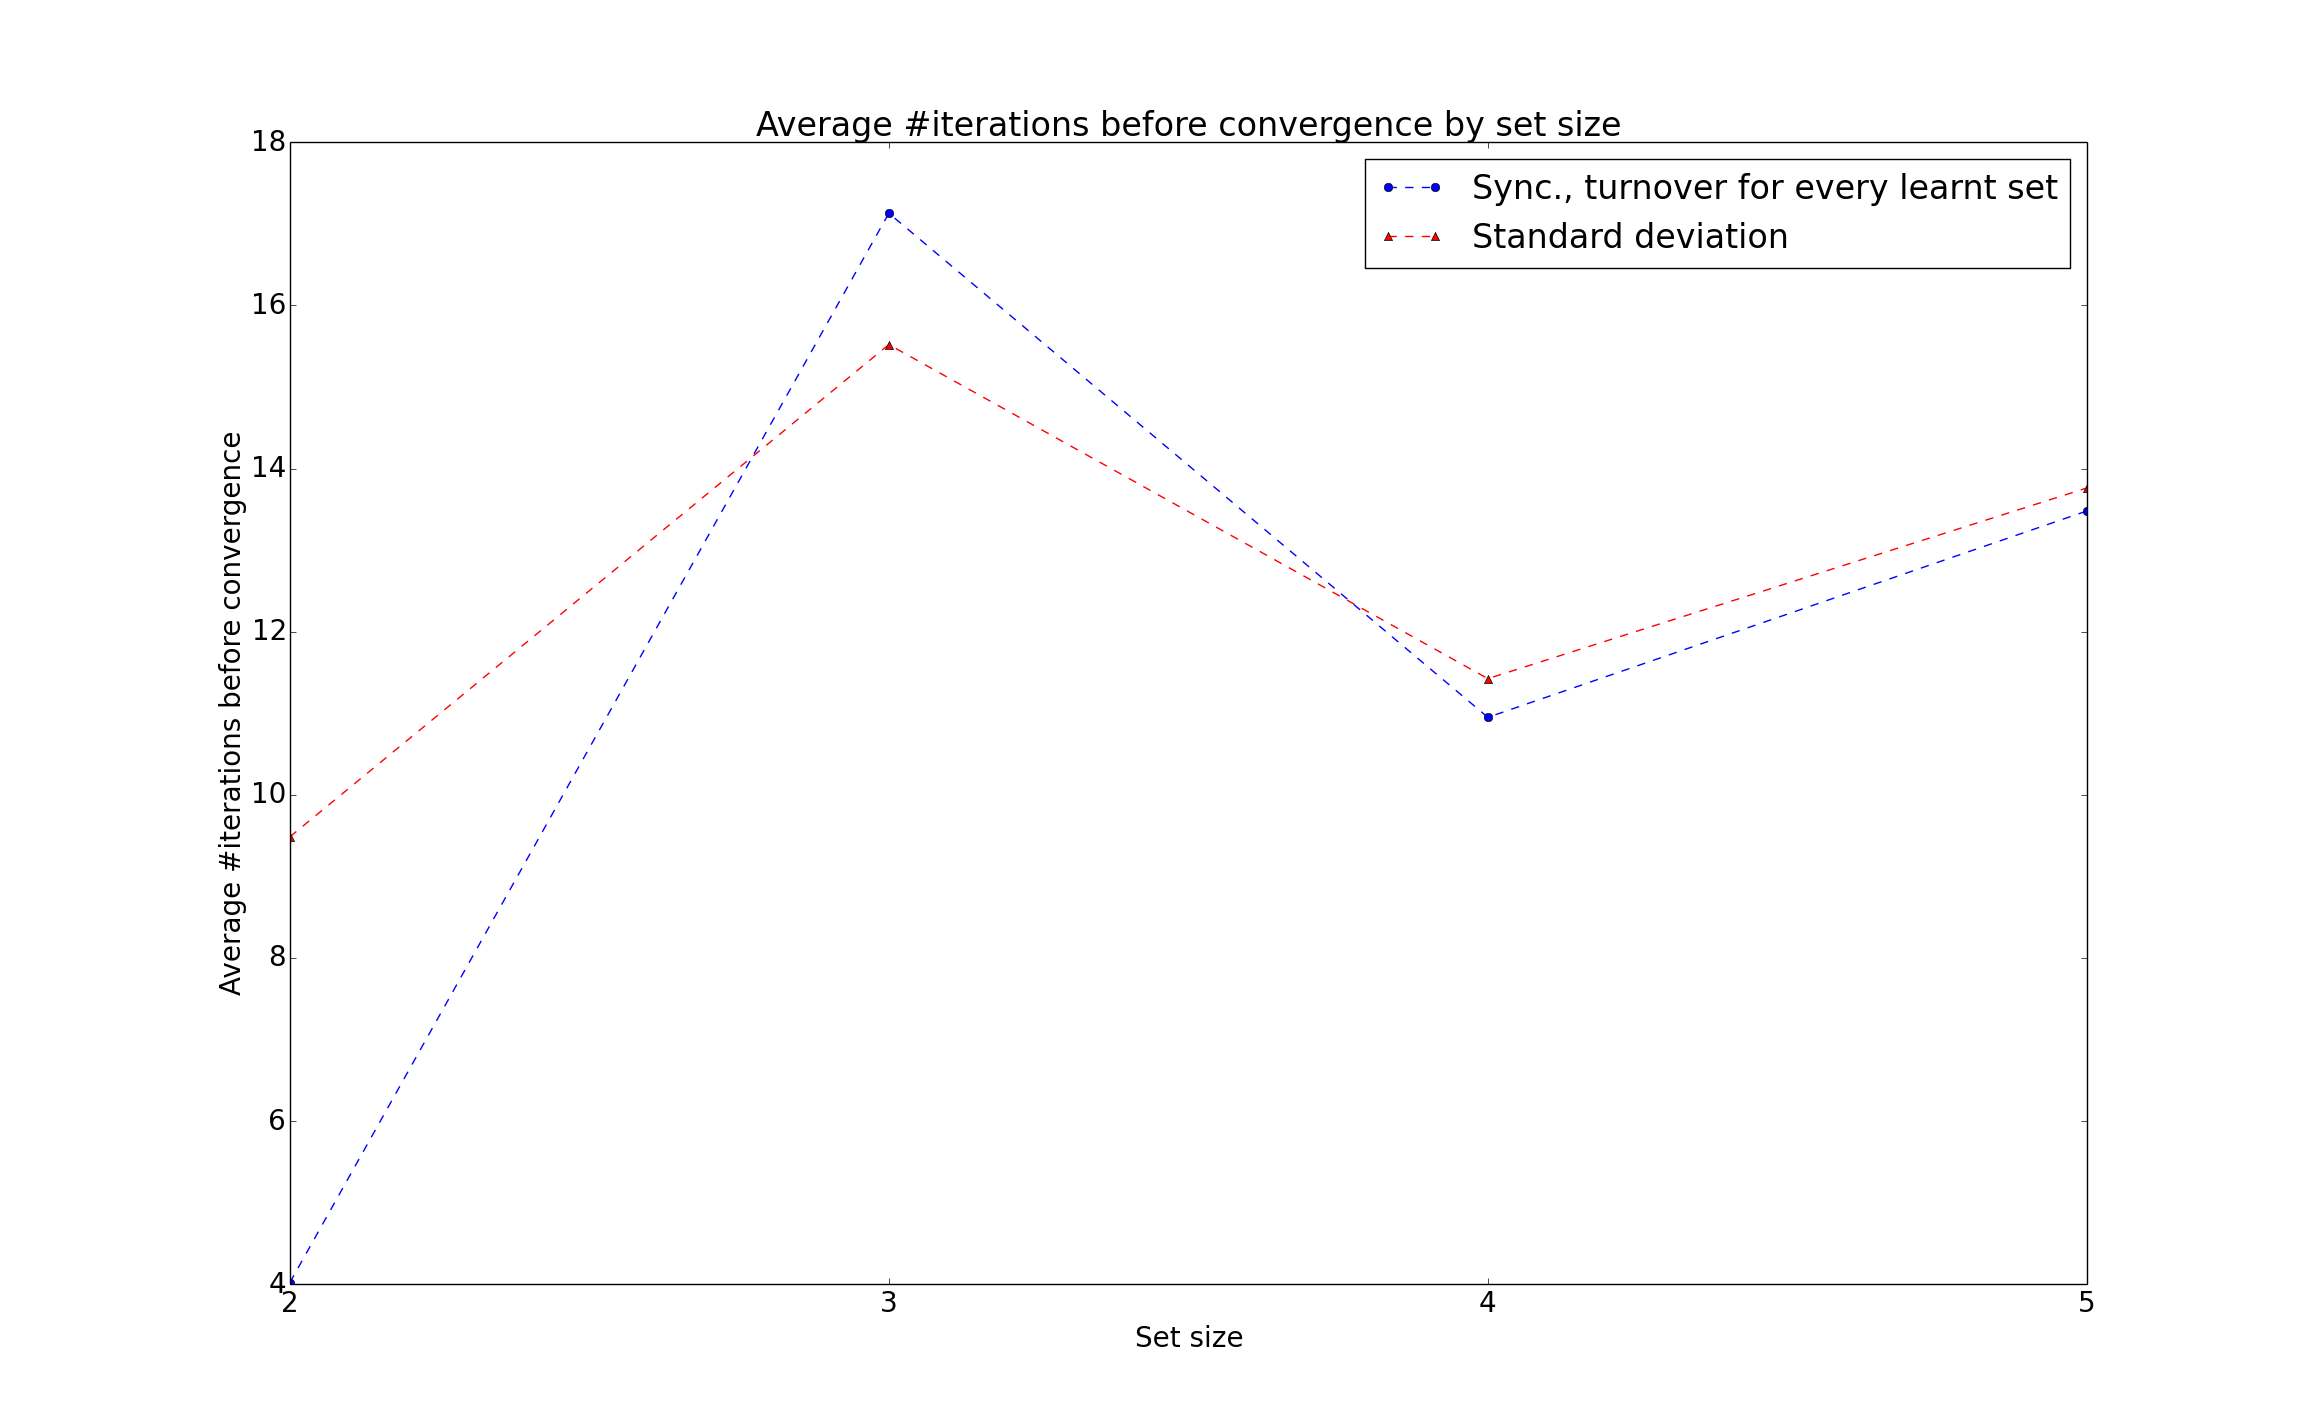
\includegraphics[width=13cm]{fig/avg_convergence_iterations_sync_mode_0.png}
%     \caption{avg iters to convergence, most successful; sync mode 0}
%     \label{fig:avg_convergence_iterations_sync_mode_0}
% \end{figure}

% \begin{figure}[h!]
%     \centering
%     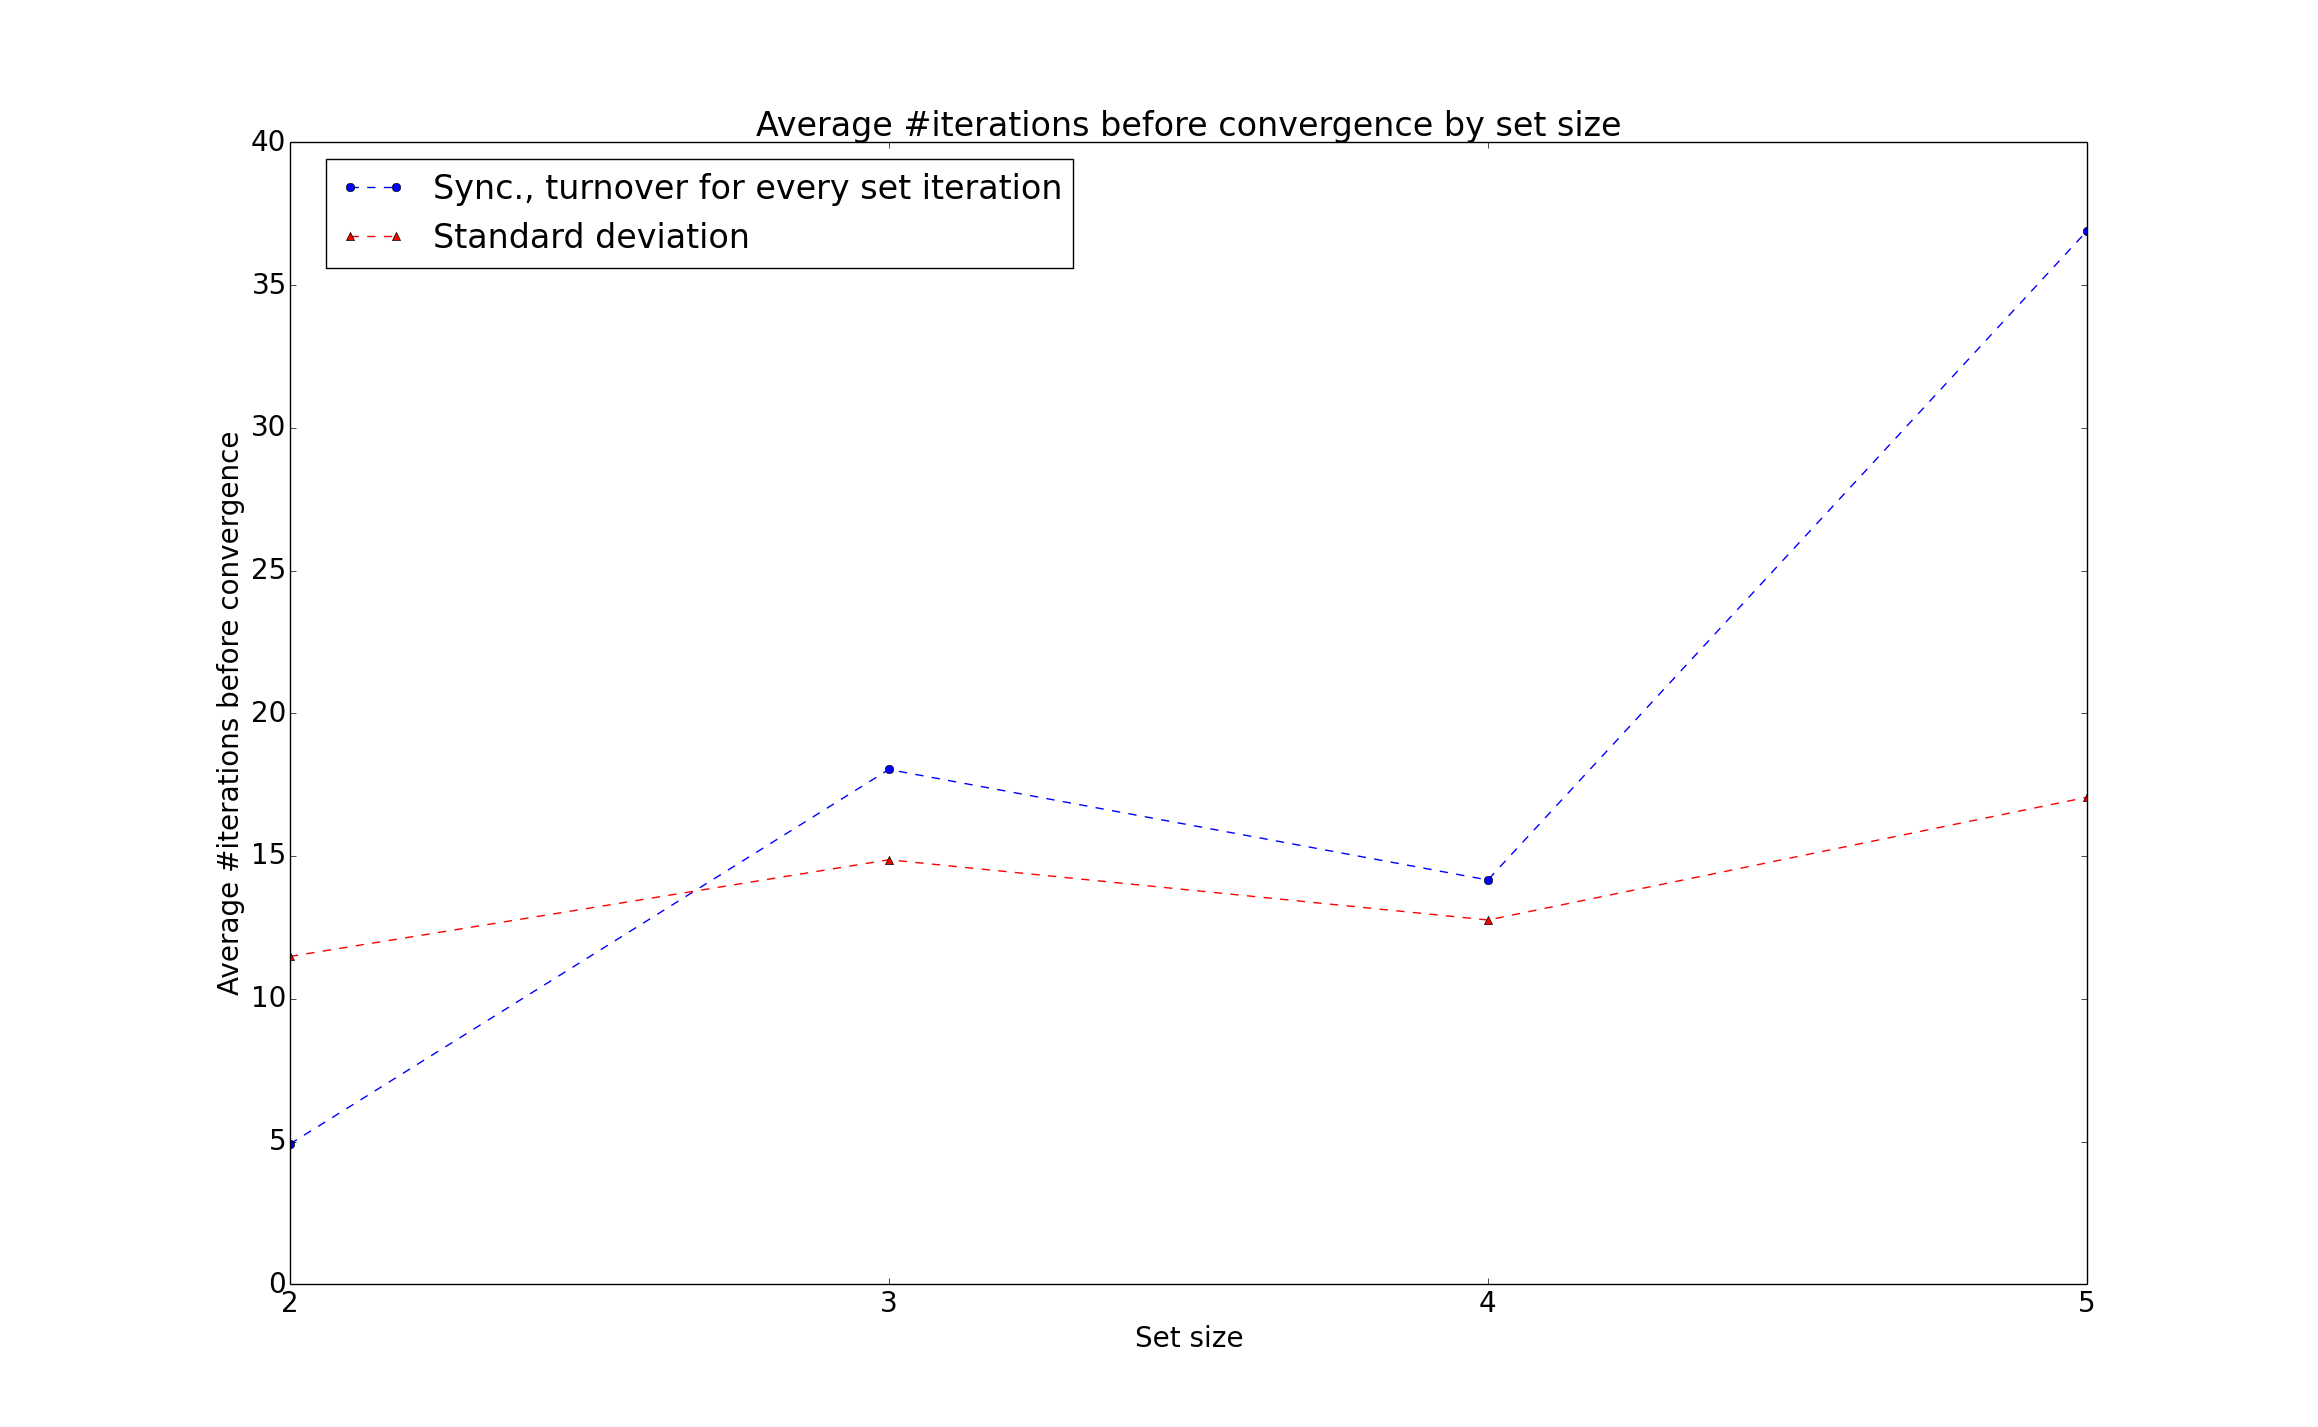
\includegraphics[width=13cm]{fig/avg_convergence_iterations_sync_mode_1.png}
%     \caption{avg iters to convergence, most successful; sync mode 1}
%     \label{fig:avg_convergence_iterations_sync_mode_1}
% \end{figure}

\begin{figure}[h!]
    \centering
    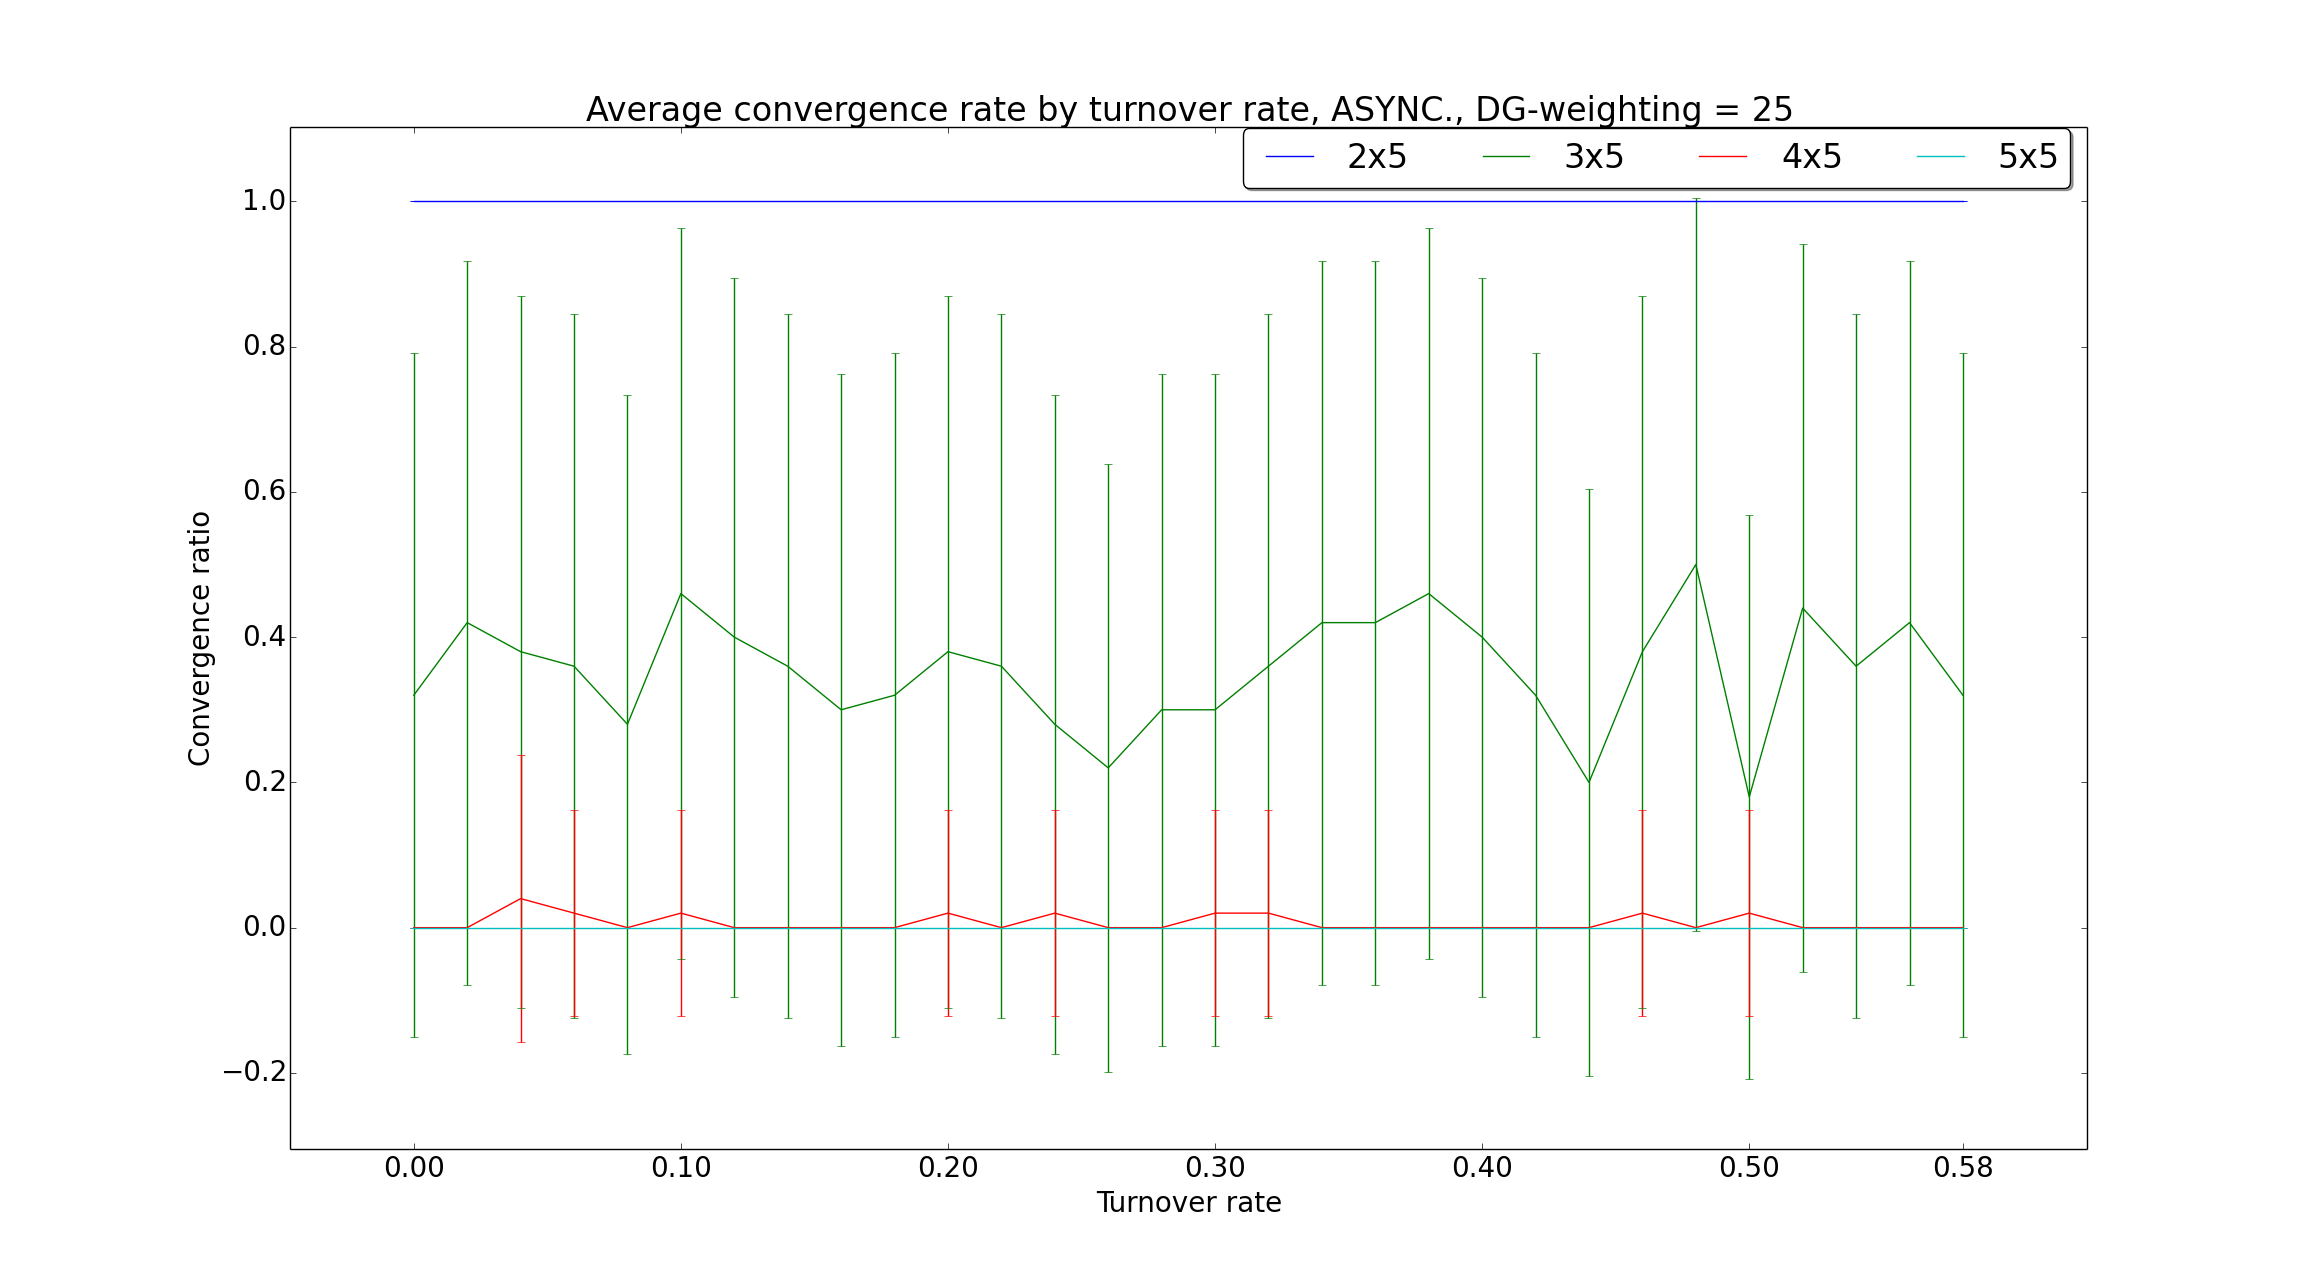
\includegraphics[width=14cm]{fig/avg_convergence_by_turnover_rate_async_dgw_25.png}
    \caption{avg convergence by turnover rate, async, dgw 25. note that it does not seem to impact this configuration - possibly async altogether. need to analyse changing the turnover rate for dgw 1, and also dgw for turnover rate 0.5 and 0.04}
    \label{fig:avg_convergence_by_turnover_rate_async_dgw_25}
\end{figure}

\begin{figure}[h!]
    \centering
    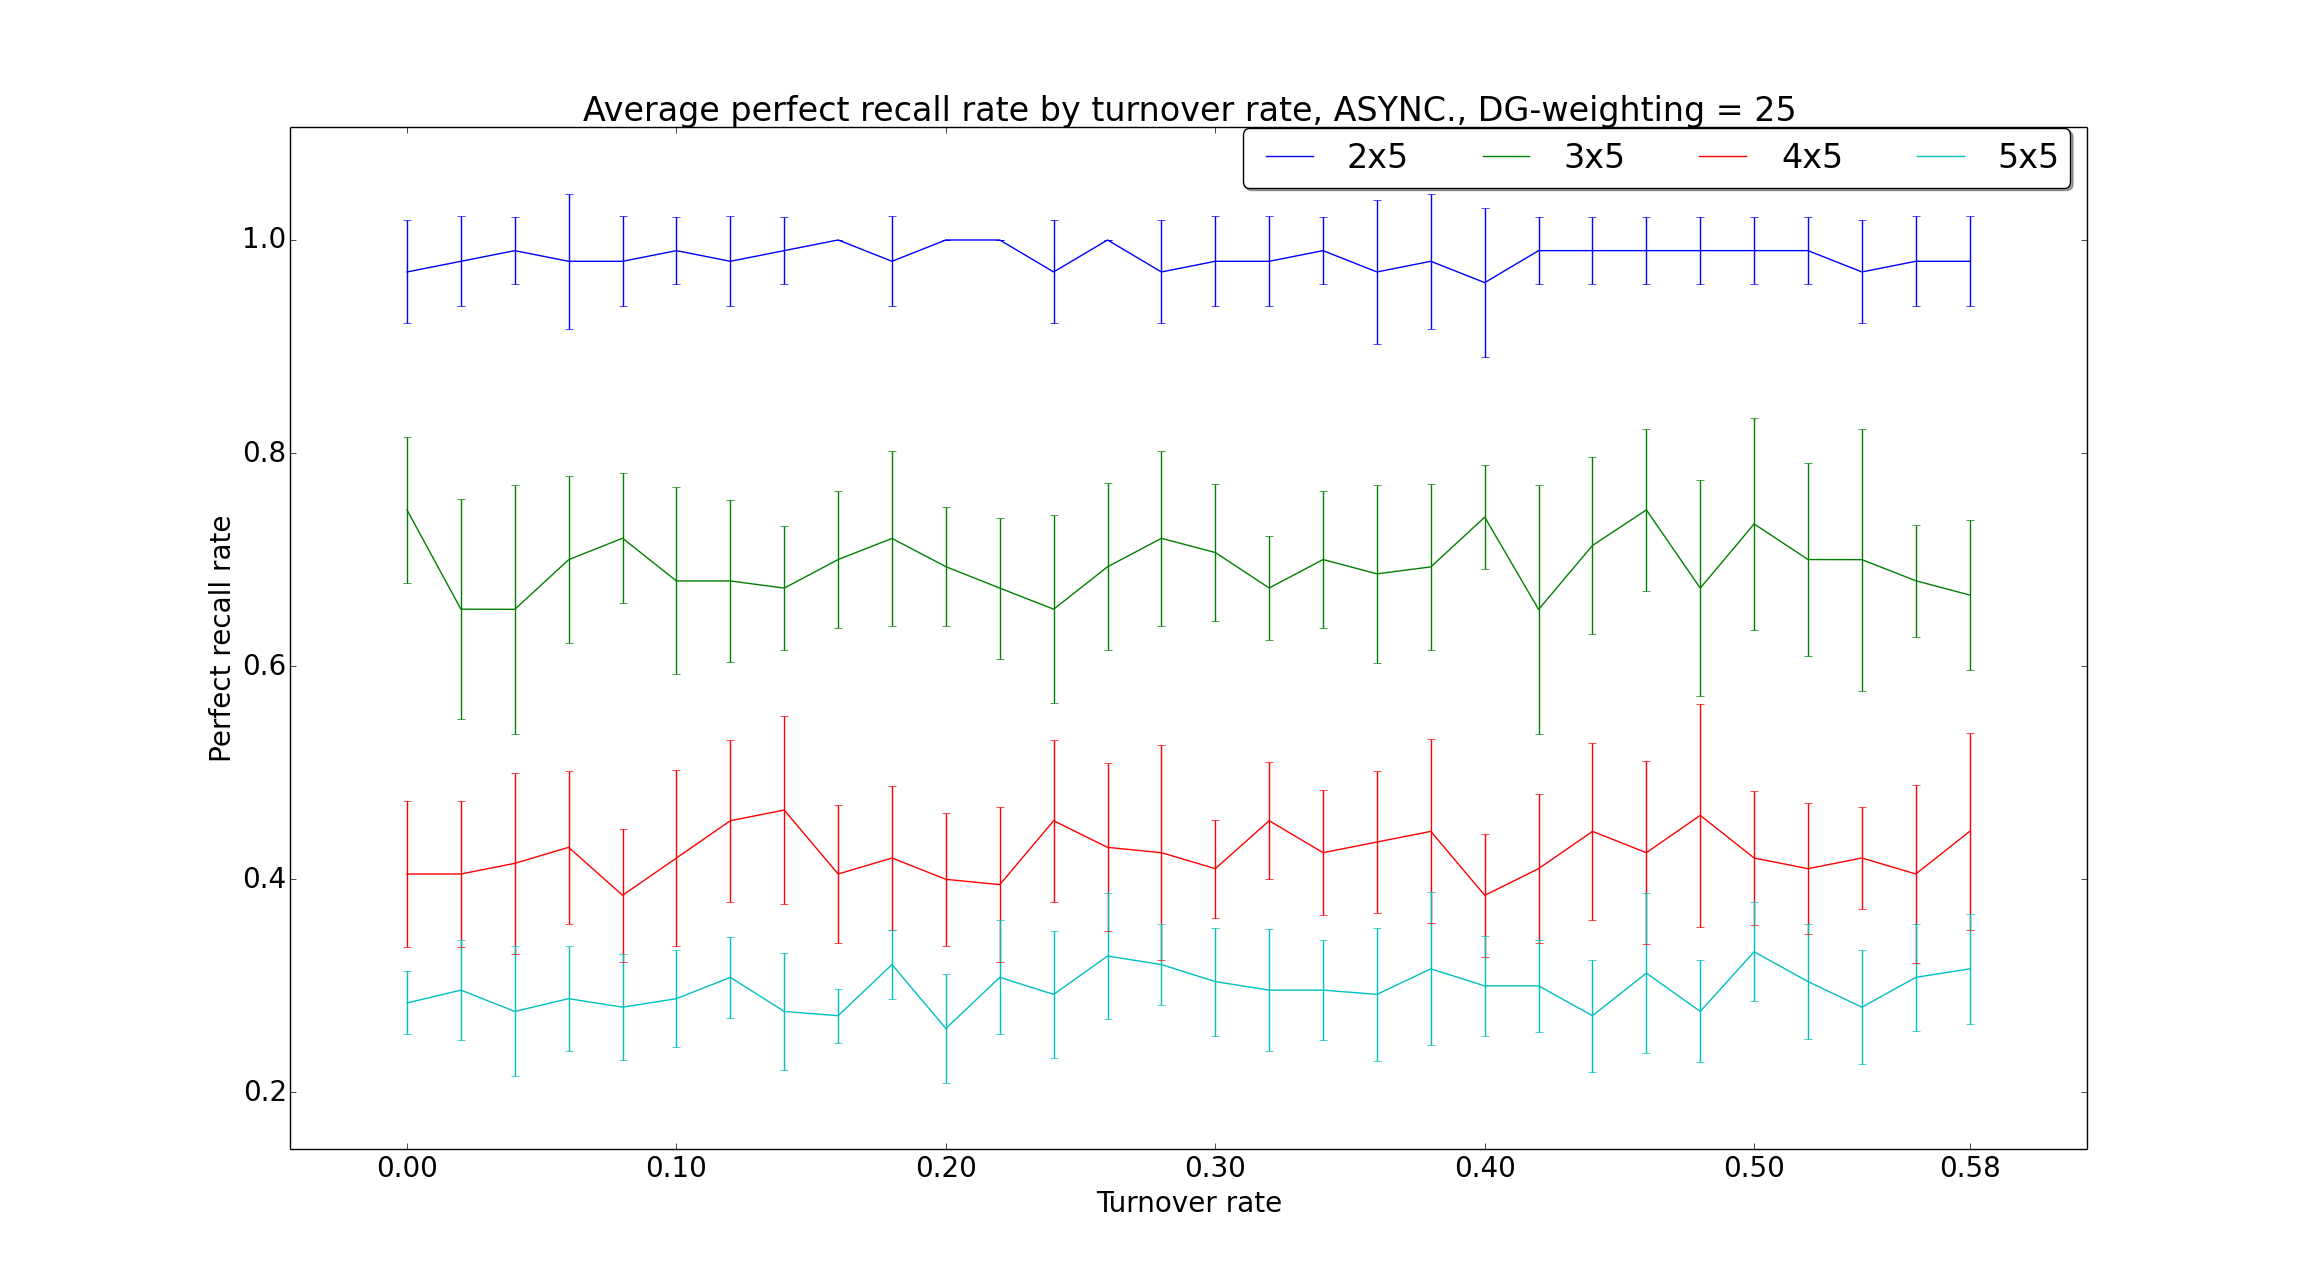
\includegraphics[width=14cm]{fig/avg_perfect_recall_rate_by_turnover_rate_async_dgw_25.png}
    \caption{avg perfect recall rate by turnover rate. note that it does not seem to impact the p.r.r. - see figure above. possibly async removes the impact this may have, although not successfully separating the given patterns - though increasing perfect recall for smaller set sizes when successful separation occurs.}
    \label{fig:avg_perfect_recall_rate_by_turnover_rate_async_dgw_25}
\end{figure}

\begin{figure}
    \centering
    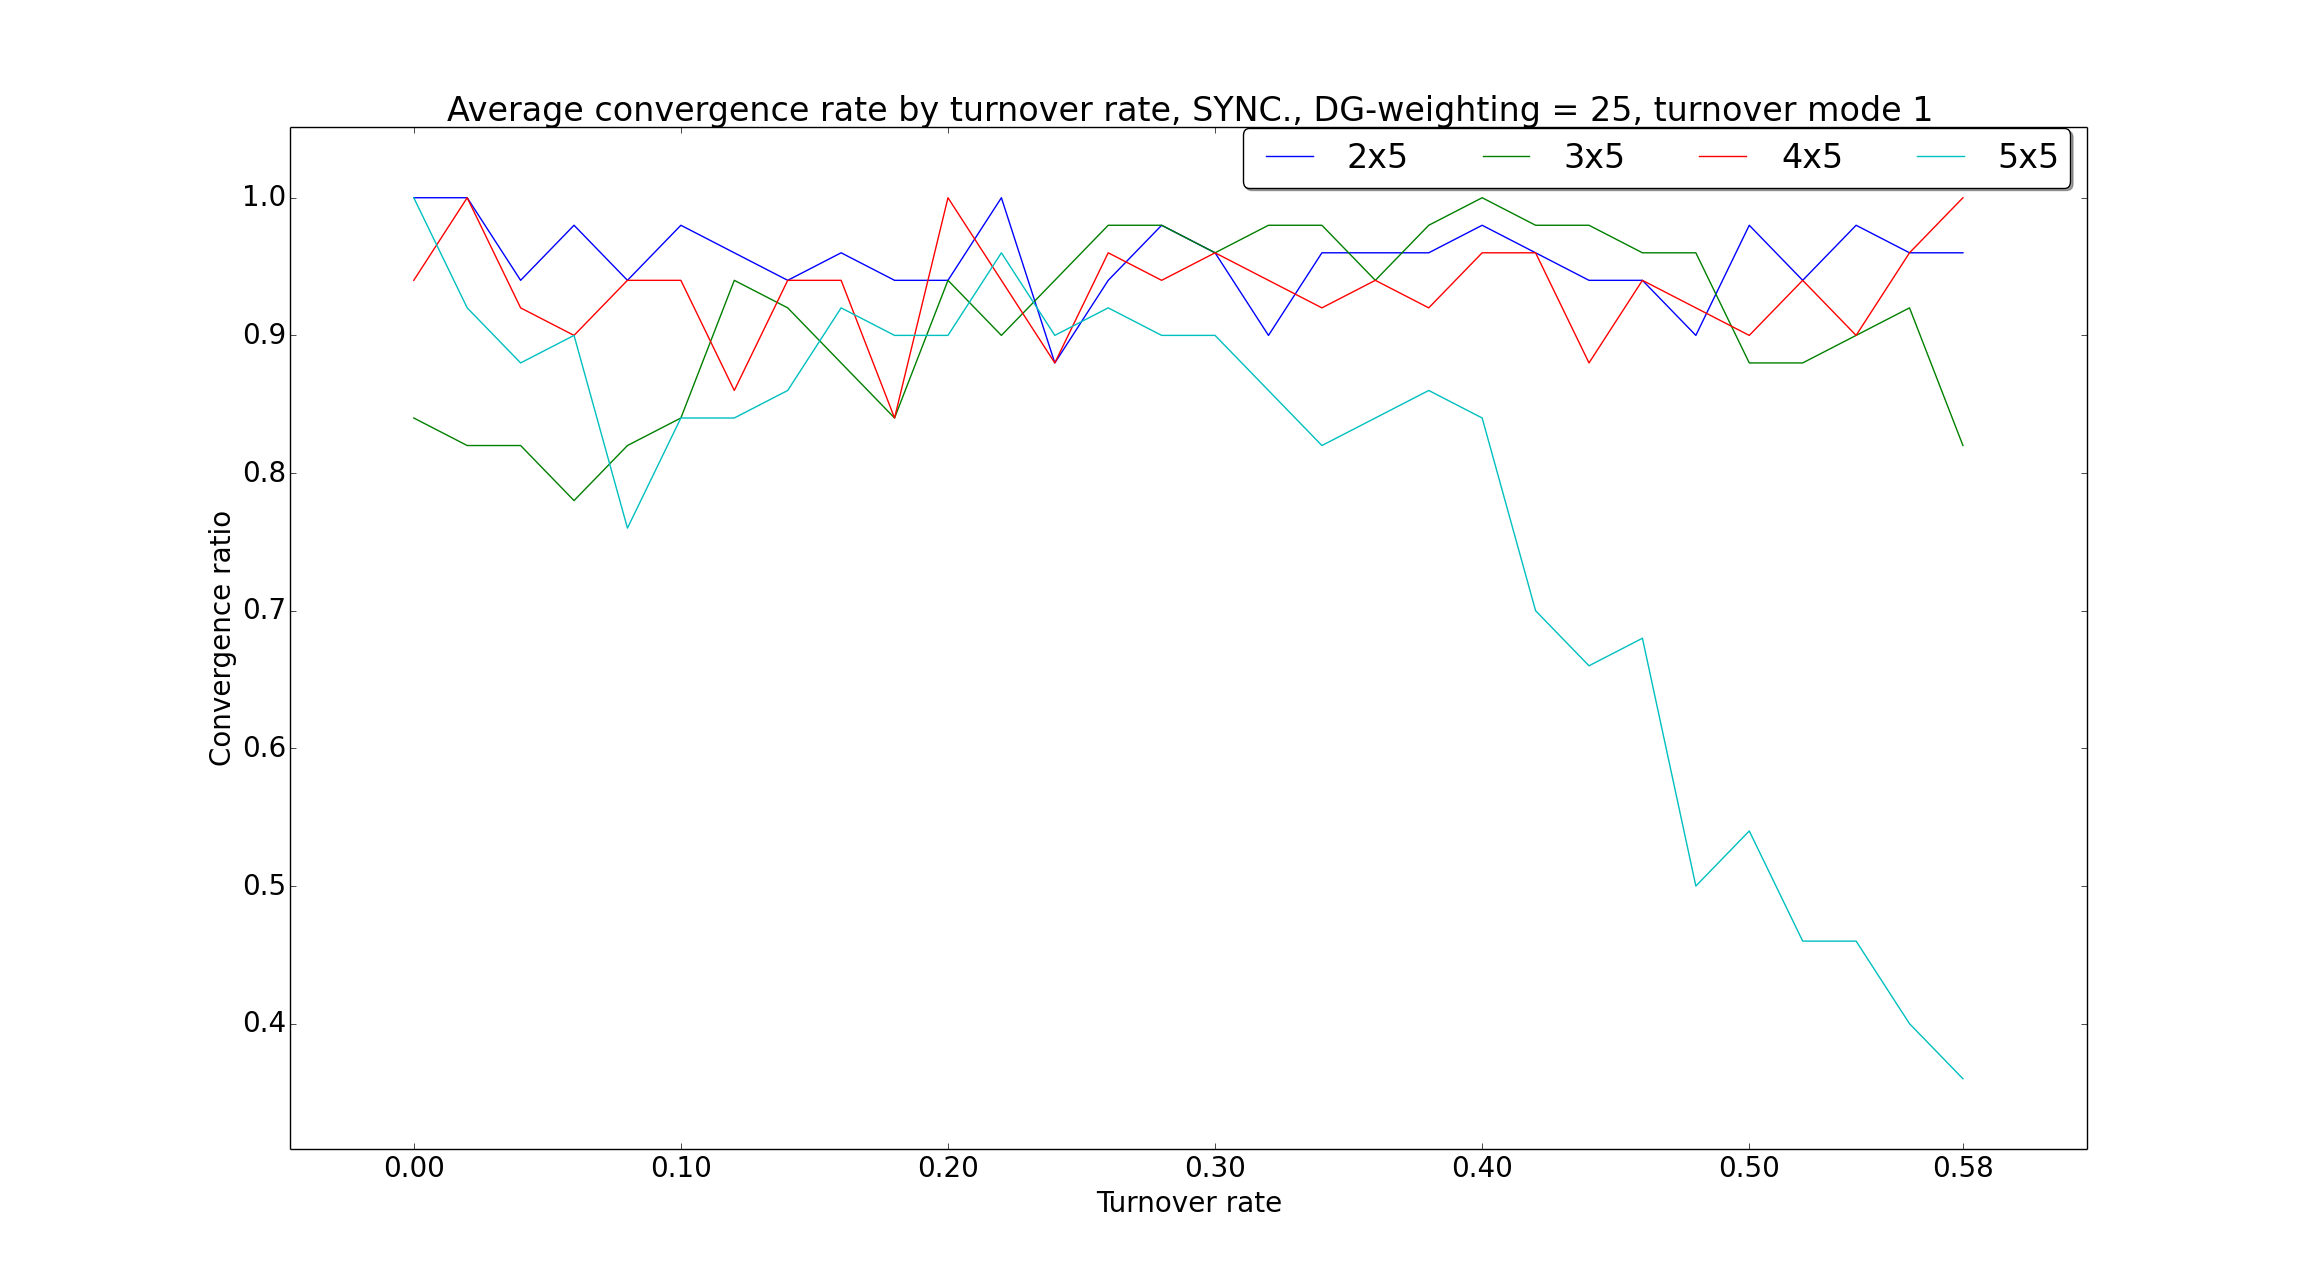
\includegraphics[width=14cm]{fig/avg_convergence_by_turnover_rate_sync_dgw_25_t_m_1_no_err_bars}
    \caption{avg convergence by turnover rate. updating scheme ca3: synchronised. dentate gyrus weighting: 25, turnover mode: 1, i.e. turnover for every new set. no err bars}
    \label{fig:avg_convergence_by_turnover_rate_sync_dgw_25_t_m_1_no_err_bars}
\end{figure}

\begin{figure}
    \centering
    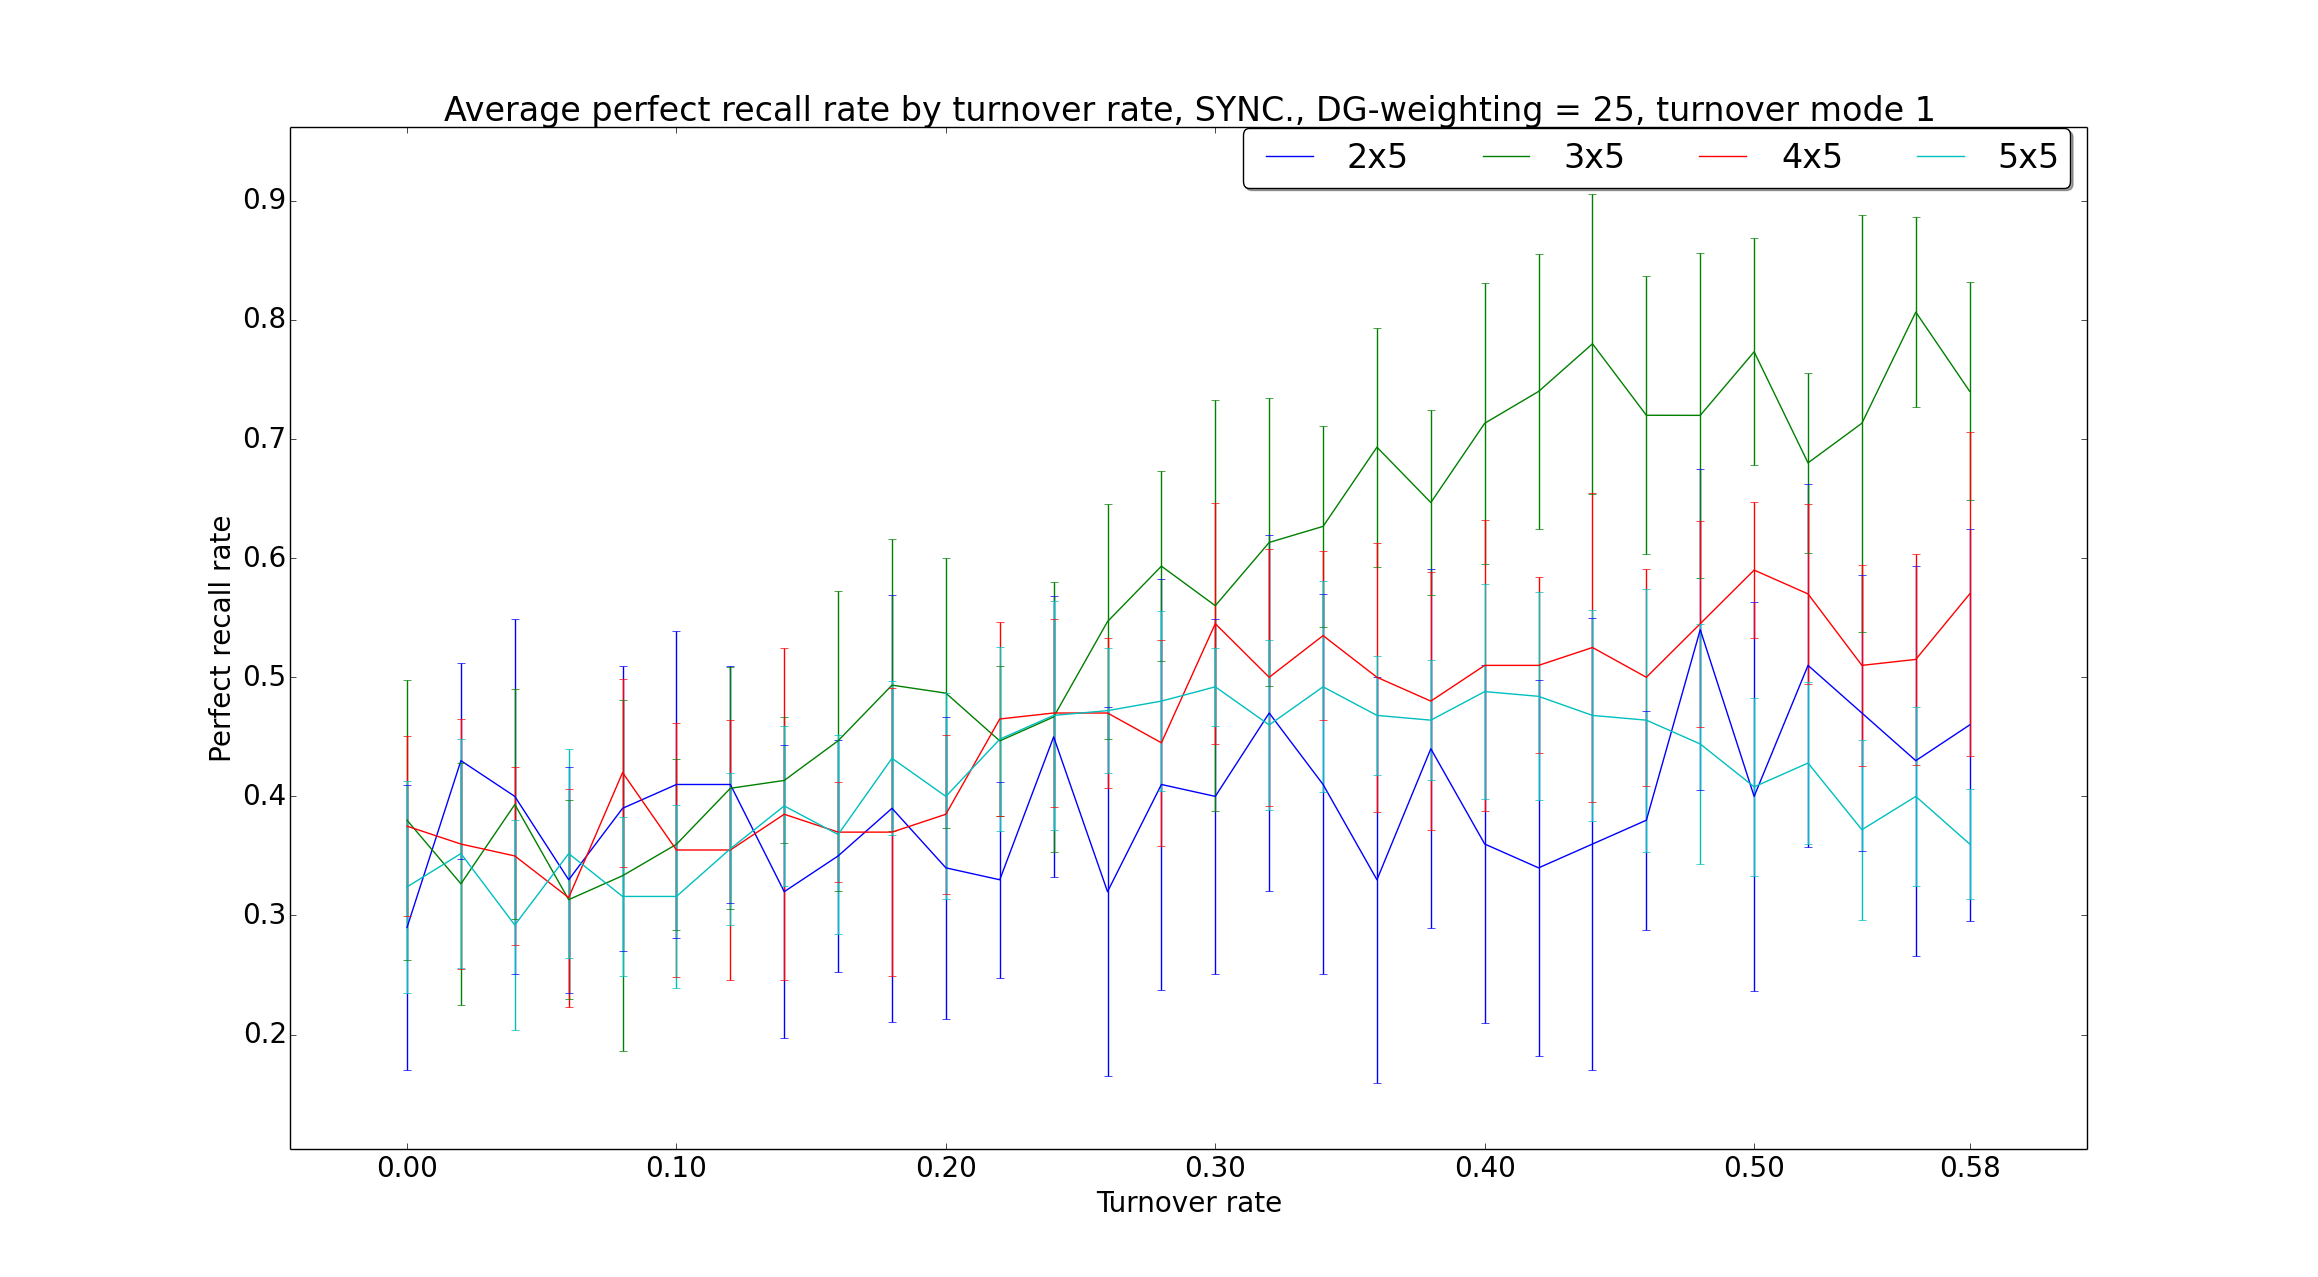
\includegraphics[width=14cm]{fig/average_perfect_recall_rates_by_set_size_sync_dgw_25_t_m_1}
    \caption{avg perfect recall rate by turnover rate. updating scheme ca3: synchronised. dentate gyrus weighting: 25, turnover mode: 1, i.e. turnover for every new set. no err bars}
    \label{fig:average_perfect_recall_rates_by_set_size_sync_dgw_25_t_m_1}
\end{figure}

\subsection{Experiment 2: Hippocampal model calibration}
\subsubsection{Methods}
\subsubsection{Results}

\subsection{Experiment 3: Extracting auto-associative patterns by chaotic recall}
\subsection{Experiment 4: Extracting hetero-associative patterns by chaotic recall}

\subsection{Experiment 5: Consolidation performance, experiment 3}
\subsection{Experiment 6: Consolidation performance, experiment 4}

\subsection{Experiment Y: Novel}

some patterns may be recalled after the next training set has been learned. i allowed this to put the pattern in the set of chaotically recalled patterns, because it reflects something which is fairly stable in the hippocampal module.
\\

Async. seems to be by far the most accurate in terms of perfect recall when it converges. Sync. with turnover for every learnt set has the highest convergence rate - non-changing for different set sizes, but the worst perfect recall rate.

It would be very interesting to see how using the 'spurious' patterns along with the actual matching patterns would consolidate to the neocortical network, comparing this to the performance attained by using the formerly outlined pseudopattern generation. In the event of having a similar effect from pattern consolidation using spurious patterns, this may point in the direction of spontaneously generated 'spurious' patterns in fact possibly acting as pseudopatterns, thus outlining a process for pseudopattern generation in the brain. (Where the stability during recall could determine the consolidation strength. For complete convergence during training using async, mode 0, about 7 iterations were required for convergence - which is thought to be (?) the number of required iterations for successful neocortical memory consolidation. This could be a spurious correlation - however, the number is equal during convergence for set size 2. If the same number of iteration can be required for a successful configuration for set size 3, this would suggest that the number is not spurious.)
\\

Along with the spurious patterns, if considering the sum of distinct perfectly recalled patterns and spurious patterns as containing information about the number of patterns, the asynchronous scheme seems to contain the most information, only falling off at set size 5. This is most likely due to the convergence being 0 \% , which it actually is at set size 4, too. Increasing the number of iterations may remedy this - however, a further calibration is most likely more relevant.
\\

The recall rate is much better for the same convergence rate in the asynchronous scheme, which points towards this being the preferable scheme. Furthermore, because turnover for every set iteration remains biologically implausible, a more plausible, yet still unrealistic model should be chosen. I.e. Async., turnover for every new set.

STD only log() in async. -> points to more stable/realistic mechanism?
\\

Gradual exposure through the constant output of the HPC during recall and learning? If this may consolidate something to the PFC, it would be really interesting.
\\

In order to target the black-box analysis that analyzing an ANN can be - particularly for the case of biologically realistic networks using chaotic neurons - I employed a type of logging, from which data is parsed, and sorted by a parser that I wrote. This data includes the number of spurious patterns extracted, where spurious is defined as not perfectly overlapping any of the provided training patterns. Furthermore, it includes the number of iterations before convergence, where 50 iterations is considered as failure to converge. It also includes the weighting selected for the connections from the DG, the neuronal turnover rate that was employed, and lastly the number of extracted patterns, along with the perfect recall rate for the current experiment.
\\

appears to be a significant correlation between the convergence rate and the perfect recall rate. this probably correlates with most positive emergent attributes that we wish to attain in the HPC network


% \begin{figure}
% \centering
% \includegraphics{fig/}
% \caption{Caption}
% \label{fig:my_label}
% \end{figure}


% ========================== section ============================
Experiment design
Results
Comparisons

\section*{Notes}

Enforce sparsity through weight updates corresponding only to the winners of kWTA - didn't work.

\textbf{100 \% connection ratio EC-CA3:}

Fairly rapid convergence for three patterns in HPC-module for turnover between every training set iteration. 
Not necessarily successful recall of all patterns. Does this have something to do with the synchronized CA3-layer during recall? Separation possible during recall when the desired pattern(s) are presented to the network - however, not all may be recalled.

-> New random pattern each time stability was reached resulted in better recall.

Is this also the case for heavier weighting of the DG-CA3 path during learning?

Spurious pattern reduction/correlation with occurrence when using turnover?

Convergence when turnover is removed between set iterations?

Heavier weighting DG. Based on paper \citep{Norman2003}. Empirical results. Chpt. 4. Figures. Nice.

\section*{Model calibration}

Experiments designed for model calibration

Dimensions analyzed outlined above.

First: STM-network extraction rate (at first, empirically observed to be same as solely auto-associative Hopfield network).


\textbf{Notes}

experiments suite - two as outlined by \citep{Hattori2014}, originally retrieved from ... as outlined above
enabling several trials automatically.

Turnover between every training set iteration (?). Needs to include empirical data on decision making. Move to preliminary experimentation in chpt. 4?
\\

It would be interesting to see HPC expanded to include neo. nets activity fed back into the hpc net. in order to induce activity. Perhaps this may cycle through previous patterns. Expanding the model towards Wakagi (08), and using a kind of reverberation could be a focal point in future work.


\cleardoublepage